% !TEX root = ../ComputationalOTFnT.tex

\chapter{Entropic Regularization of Optimal Transport}
\label{c-entropic}

This chapter introduces a family of numerical schemes to approximate solutions to Kantorovich formulation of optimal transport and its many generalizations. It operates by adding an entropic regularization penalty to the original problem. This regularization has several important advantages, which make it, when taken altogether, a very useful tool: the minimization of the regularized problem can be solved using a simple alternate minimization scheme; that scheme translates into iterations that are simple matrix-vector products, making them particularly suited to execution of GPU; for some applications, these matrix-vector products do not require storing an $n\times m$ cost matrix, but instead only require access to a kernel evaluation; in the case where a large group of measures share the same support, all of these matrix-vector products can be cast as matrix-matrix products with significant speedups; the resulting approximate distance is smooth with respect to input histogram weights and positions of the Diracs and can be differentiated using automatic differentiation.

%%%%%%%%%%%%%%%%%%%%%%%%%%%%%%%%%%%%%%%%%%%
\section{Entropic Regularization}

The discrete entropy of a coupling matrix is defined as
\eql{\label{eq-discr-entropy}
	\HD(\P) \eqdef -\sum_{i,j} \P_{i,j} (\log(\P_{i,j})-1), 
}
with an analogous definition for vectors, with the convention that $\HD(\a) = -\infty$ if one of the entries $\a_j$ is 0 or negative. The function $\HD$ is 1-strongly concave, because its Hessian is $\partial^2 \HD(P)=-\diag(1/\P_{i,j})$ and $\P_{i,j} \leq 1$. The idea of the entropic regularization of optimal transport is to use $-\HD$ as a regularizing function to obtain approximate solutions to the original transport problem~\eqref{eq-mk-discr}:
\eql{\label{eq-regularized-discr}
	\MKD_\C^\varepsilon(\a,\b) \eqdef 
	\umin{\P \in \CouplingsD(\a,\b)}
		\dotp{\P}{\C} - \varepsilon \HD(\P). 
} 
Since the objective is an $\varepsilon$-strongly convex function, Problem (\ref{eq-regularized-discr}) has a unique optimal solution. The idea to regularize the optimal transport problem by an entropic term can be traced back to modeling ideas in transportation theory~\citep{wilson1969use}: Actual traffic patterns in a network do not agree with those predicted by the solution of the optimal transport problem. Indeed, the former are more diffuse than the latter, which tend to rely on a few routes as a result of the sparsity of optimal couplings for~\eqref{eq-mk-discr}. To mitigate this sparsity, researchers in transportation proposed a model, called the ``gravity'' model~\citep{erlander1980optimal}, that is able to form a more ``blurred'' prediction of traffic given marginals and transportation costs.

Figure~\ref{fig-impact-eps} illustrates the effect of the entropy to regularize a linear program over the simplex $\simplex_3$ (which can thus be visualized as a triangle in two dimensions). Note how the entropy pushes the original LP solution away from the boundary of the triangle. The optimal $\P_\varepsilon$ progressively moves toward an ``entropic center'' of the triangle. This is further detailed in the proposition below. The convergence of the solution of that regularized problem toward an optimal solution of the original linear program has been studied by~\citet{CominettiAsympt}, with precise asymptotics.


\begin{figure}[h!]
\centering
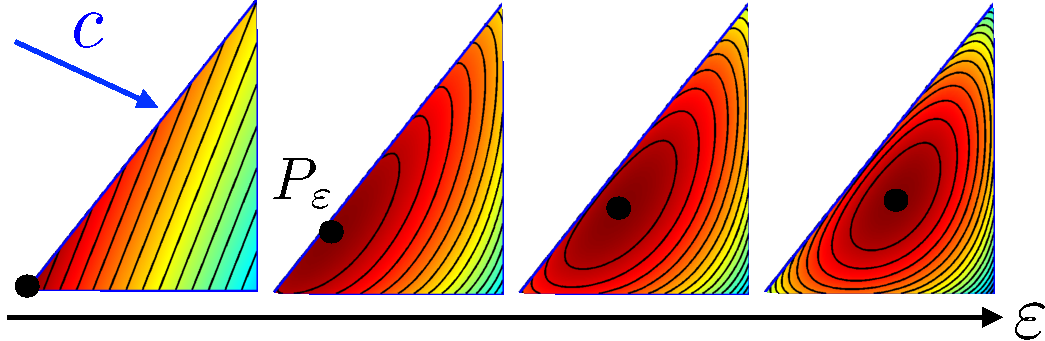
\includegraphics[width=.7\linewidth]{entropic/simplex}
\caption{\label{fig-impact-eps}
Impact of $\varepsilon$ on the optimization of a linear function on the simplex, solving $\P_\varepsilon = \argmin_{\P \in \simplex_3} \dotp{\C}{\P}-\varepsilon\HD(\P)$ for a varying $\varepsilon$. 
}
\end{figure}


\begin{prop}[Convergence with $\varepsilon$]\label{prop-convergence-eps}
The unique solution $\P_\varepsilon$ of~\eqref{eq-regularized-discr} converges to the optimal solution with maximal entropy within the set of all optimal solutions of the Kantorovich problem, namely
\eql{\label{eq-entropy-conv-1}
	\P_\varepsilon \overset{\varepsilon \rightarrow 0}{\longrightarrow}
	\uargmin{\P} \enscond{ -\HD(\P) }{
		\P \in \CouplingsD(\a,\b), \dotp{\P}{\C} = \MKD_\C(\a,\b),
	}
}
so that in particular
\eq{
	\MKD_\C^\varepsilon(\a,\b) \overset{\varepsilon \rightarrow 0}{\longrightarrow} \MKD_\C(\a,\b).
}
One also has
\eql{\label{eq-entropy-conv-2}
	\P_\varepsilon \overset{\varepsilon \rightarrow \infty}{\longrightarrow}
	\a \otimes \b = \a \transp{\b} = (\a_i \b_j)_{i,j}.
}
\end{prop}
\begin{proof}
	 We consider a sequence $(\varepsilon_\ell)_\ell$ such that $\varepsilon_\ell \rightarrow 0$ and $\varepsilon_\ell > 0$.	
 	We denote $\P_\ell$ the solution of~\eqref{eq-regularized-discr} for $\varepsilon=\varepsilon_\ell$. 
	%
	Since $\CouplingsD(\a,\b)$ is bounded, we can extract a sequence (that we do not relabel for the sake of simplicity) such that $\P_\ell \rightarrow \P^\star$. Since $\CouplingsD(\a,\b)$ is closed, $\P^\star \in \CouplingsD(\a,\b)$. We consider any $\P$ such that $\dotp{\C}{\P} = \MKD_\C(\a,\b)$. By optimality of $\P$ and $\P_\ell$ for their respective optimization problems (for $\varepsilon=0$ and $\varepsilon=\varepsilon_\ell$), one has
 	\eql{\label{eq-proof-gamma-conv}
 		0 \leq \dotp{\C}{\P_\ell} - \dotp{\C}{\P} \leq \varepsilon_\ell ( \HD(\P_\ell)-\HD(\P) ).
 	}
 	Since $\HD$ is continuous, taking the limit $\ell \rightarrow +\infty$ in this expression shows that 
 	$\dotp{\C}{\P^\star} = \dotp{\C}{\P}$ so that $\P^\star$ is a feasible point of~\eqref{eq-entropy-conv-1}. Furthermore, dividing by $\varepsilon_\ell$ in~\eqref{eq-proof-gamma-conv} and taking the limit shows that 
 	$\HD(\P) \leq \HD(\P^\star)$, which shows that $\P^\star$ is a solution of~\eqref{eq-entropy-conv-1}. Since the solution $\P_0^\star$ to this program is unique by strict convexity of $-\HD$, one has $\P^\star = \P_0^\star$, and the whole sequence is converging. 
	%
	In the limit $\varepsilon\rightarrow+\infty$, a similar proof shows that one should rather consider the problem
	\eq{
		\umin{\P \in \CouplingsD(\a,\b)} -\HD(\P),
	}
	the solution of which is $\a \otimes \b$.
\end{proof}

Formula~\eqref{eq-entropy-conv-1} states that for a small regularization $\varepsilon$, the solution converges to the maximum entropy optimal transport coupling.
%
In sharp contrast,~\eqref{eq-entropy-conv-2} shows that for a large regularization, the solution converges to the coupling with maximal entropy between two prescribed marginals $\a,\b$, namely the joint probability between two independent random variables distributed following $\a,\b$.
%
A refined analysis of this convergence is performed in~\citet{CominettiAsympt}, including a first order expansion in $\varepsilon$ (resp., $1/\varepsilon$) near $\varepsilon=0$ (resp., $\varepsilon=+\infty$).
%
Figures~\ref{fig-entropic-densities} and~\ref{fig-entropic} show visually the effect of these two convergences. A key insight is that, as $\varepsilon$ increases, the optimal coupling becomes less and less sparse (in the sense of having entries larger than a prescribed threshold), which in turn has the effect of both accelerating computational algorithms (as we study in~\S\ref{sec-sinkhorn}) and leading to faster statistical convergence (as shown in~\S\ref{sec-entropy-ot-mmd}). 

\newcommand{\myfigSinkEps}[1]{%
\imgBox{\includegraphics[width=.23\linewidth]{sinkhorn-eps/evol-img-#1}}}
\newcommand{\myfigSinkEpsV}[1]{\includegraphics[width=.24\linewidth]{sinkhorn-eps/evol-3d-#1}}

\begin{figure}[h!]
\centering
\begin{tabular}{@{}c@{}c@{}c@{}c@{}}
\myfigSinkEps{1} &
\myfigSinkEps{3} &
\myfigSinkEps{4} &
\myfigSinkEps{5} \\
\myfigSinkEpsV{1} &
\myfigSinkEpsV{3} &
\myfigSinkEpsV{4} &
\myfigSinkEpsV{5} \\
$\varepsilon=10$ &
$\varepsilon=1$ &
$\varepsilon=10^{-1}$ &
$\varepsilon=10^{-2}$ 
\end{tabular}
\caption{\label{fig-entropic-densities}
Impact of $\varepsilon$ on the couplings between two 1-D densities, illustrating Proposition~\ref{prop-convergence-eps}.
%
Top row: between two 1-D densities. Bottom row: between two 2-D discrete empirical densities with the same number $n=m$ of points (only entries of the optimal $(\P_{i,j})_{i,j}$ above a small threshold are displayed as segments between $x_i$ and $y_j$).
}
\end{figure}


\begin{figure}[h!]
\centering
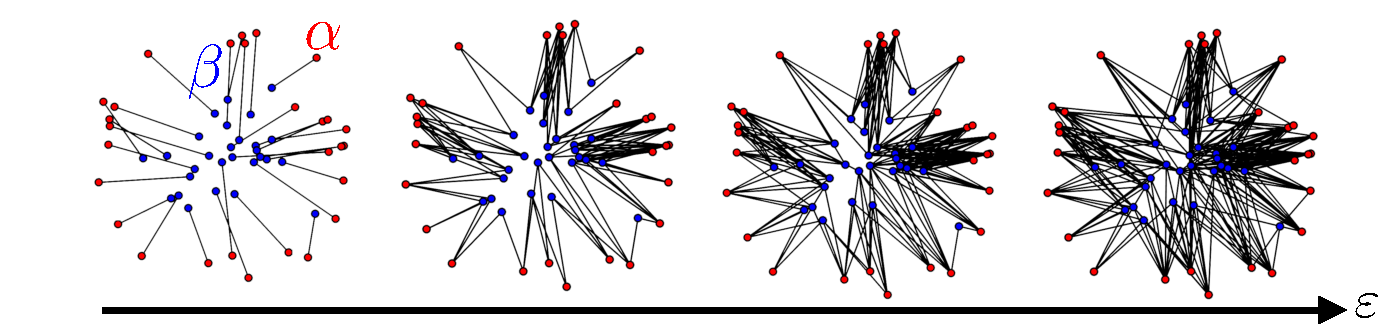
\includegraphics[width=\linewidth]{entropic/matching-2d}
\caption{\label{fig-entropic}
Impact of $\varepsilon$ on coupling between two 2-D discrete empirical densities with the same number $n=m$ of points (only entries of the optimal $(\P_{i,j})_{i,j}$ above a small threshold are displayed as segments between $x_i$ and $y_j$).
}
\end{figure}

Defining the Kullback--Leibler divergence between couplings as
\eql{\label{eq-kl-defn}
	\KLD(\P|\K) \eqdef \sum_{i,j}  \P_{i,j} \log\pa{\frac{\P_{i,j}}{\K_{i,j}}} - \P_{i,j} + \K_{i,j},
}
the unique solution $\P_\varepsilon$ of~\eqref{eq-regularized-discr} is a projection onto $\CouplingsD(\a,\b)$ of the Gibbs kernel associated to the cost matrix $\C$ as
\eq{
	\K_{i,j} \eqdef e^{-\frac{\C_{i,j}}{\varepsilon}}.
}
Indeed one has that using the definition above
\eql{\label{eq-kl-proj}
	\P_\varepsilon = \Proj_{\CouplingsD(\a,\b)}^\KLD(\K) \eqdef \uargmin{\P \in \CouplingsD(\a,\b)} \KLD(\P|\K).
}




%%%%%
\begin{rem1}{Entropic regularization between discrete measures}\label{rem:entrop-reg}
For discrete measures of the form~\eqref{eq-discr-meas}, the definition of regularized transport extends naturally to
\eql{\label{eq-entropic-disc-meas}
	\MK_\c^\varepsilon(\al,\be) \eqdef \MKD_\C^\varepsilon(\a,\b), 
} 
with cost $\C_{i,j}=\c(x_i,y_j)$, to emphasize the dependency with respect to the positions $(x_i,y_j)$ supporting the input measures.
\end{rem1}
%%%%%


%%%%%
\begin{rem2}{General formulation}
One can consider arbitrary measures by replacing the discrete entropy by the relative entropy with respect to the product measure $\d\al\otimes\d\be(x,y) \eqdef \d\al(x)\d\be(y)$, and propose a regularized counterpart to~\eqref{eq-mk-generic} using
\eql{\label{eq-entropic-generic}
	\MK_\c^\varepsilon(\al,\be) \eqdef 
	\umin{\pi \in \Couplings(\al,\be)}
		\int_{\X \times \Y} c(x,y) \d\pi(x,y) + \varepsilon \KL(\pi|\al\otimes\be),
}
where the relative entropy is a generalization of the discrete Kullback--Leibler divergence~\eqref{eq-kl-defn}
\eql{\label{eq-defn-rel-entropy}
\begin{aligned}	 \KL(\pi|\xi) \eqdef \int_{\X \times \Y} \log\Big( \frac{\d \pi}{\d\xi}(x,y) \Big) \d\pi(x,y)\\
	  + \int_{\X \times \Y} (\d\xi(x,y)-\d\pi(x,y)), 
	  \end{aligned}
}
and by convention $\KL(\pi|\xi)=+\infty$ if $\pi$ does not have a density $\frac{\d \pi}{\d\xi}$ with respect to $\xi$. 
%
It is important to realize that the reference measure $\al\otimes\be$ chosen in~\eqref{eq-entropic-generic} to define the entropic regularizing term $\KL(\cdot|\al\otimes\be)$ plays no specific role; only its support matters, as noted by the following proposition.

\begin{prop}
	For any $\pi \in \Couplings(\al,\be)$, and for any $(\al',\be')$  having the same 0 measure sets as $(\al,\be)$ (so that they have both densities with respect to one another) one has
	\eq{
		\KL(\pi|\al\otimes\be) = \KL(\pi|\al'\otimes\be') - \KL(\al\otimes\be|\al'\otimes\be').
	}
\end{prop}
\todoK{
\begin{proof}
	\todo{Prove it}
\end{proof}
}

This proposition shows that choosing $\KL(\cdot|\al'\otimes\be')$ in place of $\KL(\cdot|\al\otimes\be)$ in~\eqref{eq-entropic-generic} results in the same solution.


Formula~\eqref{eq-entropic-generic} can be refactored as a projection problem
\eql{\label{eq-entropic-generic-proj}
	\umin{\pi \in \Couplings(\al,\be)} \KL(\pi|\Kk),
}
where $\Kk$ is the Gibbs distributions $\d\Kk(x,y) \eqdef e^{-\frac{c(x,y)}{\varepsilon}} \d\mu(x)\d\nu(y)$.
%
This problem is often referred to as the ``static Schr\"odinger problem''~\citep{LeonardSchroedinger,RuschendorfThomsen}, since it was initially considered by Schr\"odinger in statistical physics~\citep{Schroedinger31}. 
%
As $\varepsilon \rightarrow 0$, the unique solution to~\eqref{eq-entropic-generic-proj} converges to the maximum entropy solution to~\eqref{eq-mk-generic}; see~\citep{leonard2012schrodinger,2017-carlier-SIMA}.
%
Section \ref{sec-entropic-dynamic} details an alternate ``dynamic'' formulation of the Schr\"odinger problem over the space of paths connecting the points of two measures.
\end{rem2}
%%%%%

%%%%%
\begin{rem2}{Mutual entropy}
Similarly to~\eqref{eq-ot-proba-interpretation}, one can re\-phra\-se \eqref{eq-entropic-generic} using random variables 
\eq{
	\MK_\c^\varepsilon(\al,\be) = \umin{(X,Y)} \enscond{ \EE_{(X,Y)}(c(X,Y)) + \epsilon \text{I}(X,Y) }{ X \sim \al, Y \sim \be },
}
where, denoting $\pi$ the distribution of $(X,Y)$, $\text{I}(X,Y) \eqdef \KL(\pi|\al\otimes\be)$ is the so-called mutual information between the two random variables. One has $\text{I}(X,Y) \geq 0$ and $\text{I}(X,Y)=0$ if and only if the two random variables are independent.  
\end{rem2}

%%%%%
\begin{rem2}{Independence and couplings}
	A coupling $\pi \in \Couplings(\al,\be)$ describes the distribution of a couple of random variables $(X,Y)$ defined on $(\X,\Y)$, where $X$ (resp., $Y$) has law $\al$ (resp., $\be$).
	% 
	Proposition~\ref{prop-convergence-eps} carries over for generic (nonnecessary discrete) measures, so that the solution $\pi_\varepsilon$ of~\eqref{eq-entropic-generic} converges to the tensor product coupling $\al \otimes \be$ as $\varepsilon \rightarrow+\infty$. This coupling $\al \otimes \be$ corresponds to the random variables $(X,Y)$ being independent. 
	%
	In contrast, as $\varepsilon \rightarrow 0$, $\pi_\varepsilon$ convergence to a solution $\pi_0$ of the OT problem~\eqref{eq-mk-generic}. On $\X=\Y=\RR^\dim$, if $\al$ and $\be$ have densities with respect to the Lebesgue measure, as detailed in Remark~\ref{rem-exist-mongemap}, then $\pi_0$ is unique and supported on the graph of a bijective Monge map $\T : \RR^\dim \rightarrow \RR^\dim$. In this case, $(X,Y)$ are in some sense fully dependent, since $Y=\T(X)$ and $X=\T^{-1}(Y)$. 
	%
	In the simple 1-D case $\dim=1$, a convenient way to visualize the dependency structure between $X$ and $Y$ is to use the copula $\xi_\pi$ associated to the joint distribution $\pi$. The cumulative function defined in~\eqref{eq-cumul-defn} is extended to couplings as 
	\eq{
		\foralls (x,y) \in \RR^2, \quad
		\cumul{\pi}(x,y) \eqdef \int_{-\infty}^x \int_{-\infty}^y \d\pi.  
	}
	The copula is then defined as
	\eq{
		\foralls (s,t) \in [0,1]^2, \quad
		\xi_{\pi}(s,t) \eqdef \cumul{\pi}( \cumul{\al}^{-1}(s),\cumul{\be}^{-1}(t) ),
	}
	where the pseudoinverse of a cumulative function is defined in~\eqref{eq-pseudo-inv-cum}. 
	%
	For independent variables, $\varepsilon=+\infty$, \ie $\pi=\al\otimes \be$, one has $\xi_{\pi_{+\infty}}(s,t)=st$.
	%
	In contrast, for fully dependent variables, $\varepsilon=+\infty$, one has $\xi_{\pi_0}(s,t)=\min(s,t)$.
	%
	Figure~\ref{fig-entropic-copula} shows how entropic regularization generates copula $\xi_{\pi_\varepsilon}$ interpolating between these two extreme cases. 
\end{rem2}
%%%%%

% G B D H
\newcommand{\myfigSinkCopul}[1]{\imgBox{\includegraphics[width=.185\linewidth,trim=65 55 45 40,clip]{sinkhorn-copula/evol-#1}}}
\begin{figure}[h!]
\centering
\begin{tabular}{@{}c@{\hspace{5mm}}c@{}}
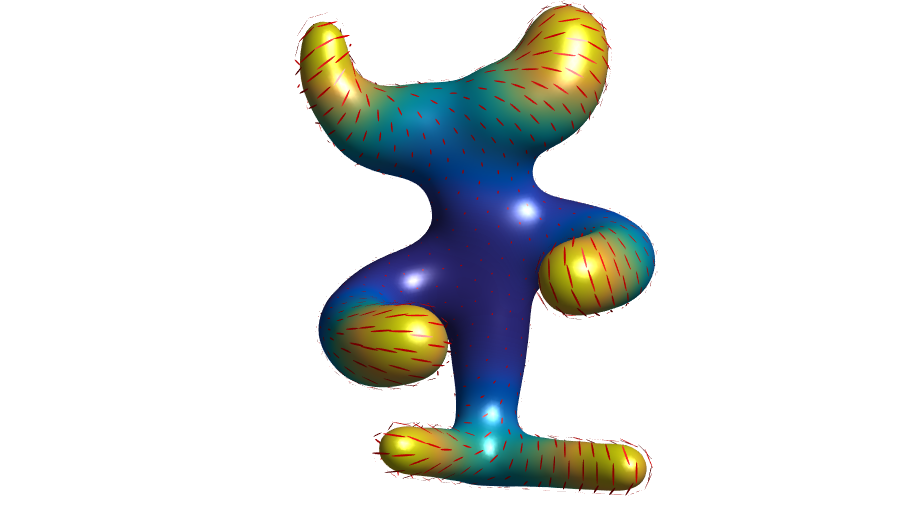
\includegraphics[width=.4\linewidth]{sinkhorn-copula/input-1} & 
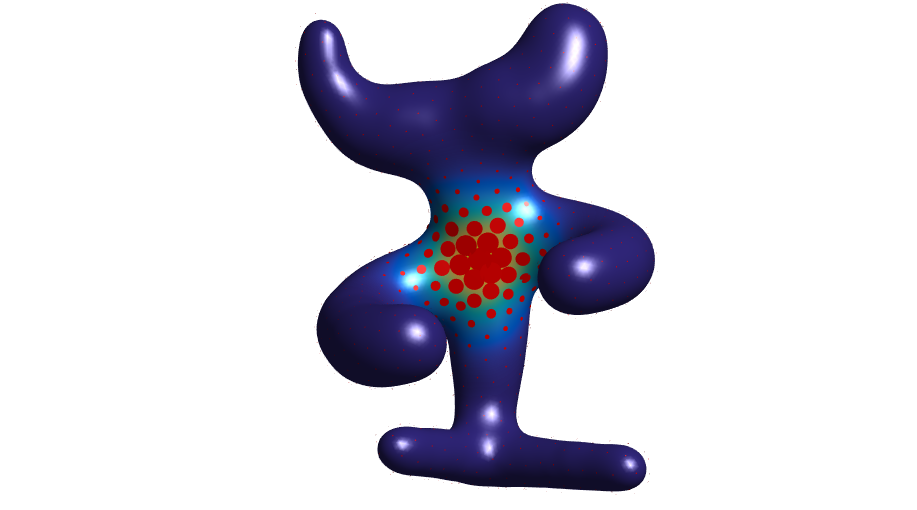
\includegraphics[width=.4\linewidth]{sinkhorn-copula/input-2}\\
{\color{red}$\al$} & {\color{blue}$\be$}
\end{tabular}
%
\begin{tabular}{@{}c@{}c@{}c@{}c@{}c@{}}
\myfigSinkCopul{levelsets-1} &
\myfigSinkCopul{levelsets-2} &
\myfigSinkCopul{levelsets-3} &
\myfigSinkCopul{levelsets-4} &
\myfigSinkCopul{levelsets-5} \\
\myfigSinkCopul{copula-1} &
\myfigSinkCopul{copula-2} &
\myfigSinkCopul{copula-3} &
\myfigSinkCopul{copula-4} &
\myfigSinkCopul{copula-5} \\
{\color[rgb]{1,0,1} $\varepsilon=10$} &
{\color[rgb]{.75,.25,.75} $\varepsilon=1$} &
{\color[rgb]{.5,.5,.5} $\varepsilon=0.5 \cdot 10^{-1}$} &
{\color[rgb]{.25,.75,.25} $\varepsilon=10^{-1}$} &
{\color[rgb]{0,1,0} $\varepsilon=10^{-3}$} 
\end{tabular}
\caption{\label{fig-entropic-copula}
Top: evolution with $\varepsilon$ of the solution $\pi_\varepsilon$ of~\eqref{eq-entropic-generic}. 
Bottom: evolution of the copula function $\xi_{\pi_\varepsilon}$. 
}
\end{figure}


%%%%%%%%%%%%%%%%%%%%%%%%%%%%%%%%%%%%%%%%%%%
\section{Sinkhorn's Algorithm and Its Convergence}
\label{sec-sinkhorn}

The following proposition shows that the solution of~\eqref{eq-regularized-discr} has a specific form, which can be parameterized using $n+m$ variables. That parameterization is therefore essentially dual, in the sense that a coupling $\P$ in $\CouplingsD(\a,\b)$ has $nm$ variables but $n+m$ constraints.

\begin{prop}\label{prop-regularized-primal}
The solution to~\eqref{eq-regularized-discr} is unique and has the form
\eql{\label{eq-scaling-form}
	\foralls (i,j) \in \range{n} \times \range{m}, \quad \P_{i,j} = \uD_i \K_{i,j} \vD_j
}
for two (unknown) scaling variable $(\uD,\vD) \in \RR_+^n \times \RR_+^m$. 
\end{prop} 

\begin{proof} 
Introducing two dual variables $\fD\in\RR^n,\gD\in\RR^m$ for each marginal constraint, the Lagrangian of~\eqref{eq-regularized-discr} reads
\eq{\label{eq-sinkhorn-lagrangian}
	\Lag(\P,\fD,\gD)= \dotp{\P}{\C} - \varepsilon \HD(\P) - \dotp{\fD}{\P\ones_m-\a}-\dotp{\gD}{\transp{\P}\ones_n-\b}.
}
First order conditions then yield
$$
	\frac{\partial\Lag(\P,\fD,\gD)}{\partial \P_{i,j}}= \C_{i,j} + \varepsilon \log(\P_{i,j}) - \fD_i -\gD_j=0,
$$
which result, for an optimal $\P$ coupling to the regularized problem, in the expression $\P_{i,j}=e^{\fD_i/\varepsilon}e^{-\C_{i,j}/\varepsilon}e^{\gD_j/\varepsilon}$, which can be rewritten in the form provided above using nonnegative vectors $\uD$ and $\vD$.
\end{proof} 

%%%
\paragraph{Regularized OT as matrix scaling.} 

The factorization of the optimal solution exhibited in Equation~\eqref{eq-scaling-form} can be conveniently rewritten in matrix form as $\P=\diag(\uD)\K\diag(\vD)$.
%
The variables $(\uD,\vD)$ must therefore satisfy the following nonlinear equations which correspond to the mass conservation constraints inherent to $\CouplingsD(\a,\b)$:
\eql{\label{eq-dualsinkhorn-constraints}
	\diag(\uD)\K\diag(\vD)\ones_m=\a,
	\qandq
	\diag(\vD)\K^\top \diag(\uD)\ones_n=\b.
}
These two equations can be further simplified, since $\diag(\vD)\ones_m$ is simply $\vD$, and the multiplication of $\diag(\uD)$ times $\K \vD$ is 
\eql{\label{eq-dualsinkhorn-constraints2}
	\uD \odot (\K \vD) = \a
	\qandq
	\vD \odot (\transp{\K}\uD) = \b,
}
where $\odot$ corresponds to entrywise multiplication of vectors. That problem is known in the numerical analysis community as the matrix scaling problem (see~\citep{nemirovski1999complexity} and references therein).
%
An intuitive way to handle these equations is to solve them iteratively, by modifying first $\uD$ so that it satisfies the left-hand side of Equation~\eqref{eq-dualsinkhorn-constraints2} and then $\vD$ to satisfy its right-hand side. These two updates define Sinkhorn's algorithm,
\eql{\label{eq-sinkhorn}	
	\itt{\uD} \eqdef \frac{\a}{\K \it{\vD}}
	\qandq
	\itt{\vD} \eqdef \frac{\b}{\transp{\K}\itt{\uD}},
}
initialized with an arbitrary positive vector $\init{\vD} = \ones_m$. The division operator used above between two vectors is to be understood entrywise. Note that a different initialization will likely lead to a different solution for $\uD,\vD$, since $\uD,\vD$ are only defined up to a multiplicative constant (if $\uD,\vD$ satisfy \eqref{eq-dualsinkhorn-constraints} then so do $\lambda\uD,\vD/\lambda$ for any $\lambda>0$).
%
It turns out, however, that these iterations converge (see Remark~\ref{rem-iterative-projection} for a justification using iterative projections, and see Remark~\ref{rem-global-conv-sinkh} for a strict contraction result) and all result in the same optimal coupling $\diag(\uD)\K\diag(\vD)$. 
%
Figure~\ref{fig-sinkhorn-convergence}, top row, shows the evolution of the coupling $\diag(\it{\uD})\K\diag(\it{\vD})$ computed by Sinkhorn iterations. It  evolves from the Gibbs kernel $\K$ toward the optimal coupling solving~\eqref{eq-regularized-discr} by progressively shifting the mass away from the diagonal.

\begin{rem}[Historical perspective] The iterations~\eqref{eq-sinkhorn} first appeared in~\citep{yule1912methods,kruithof}. They were later known as the iterative proportional fitting procedure (IPFP)~\citet{DemingStephanIPFP} and RAS~\citep{bacharach1965estimating} methods~\citep{ReviewSinkhorn}. The proof of their convergence is attributed to~\citet{Sinkhorn64}, hence the name of the algorithm. This algorithm was later extended in infinite dimensions by~\citet{Ruschendorf95}. This regularization was used in the field of economics to obtain approximate solutions to optimal transport problems, under the name of gravity models~\citep{wilson1969use,erlander1980optimal,erlander1990gravity}.
% with later contributions~\citep{SinkhornKnopp67,Sinkhorn67}
It was rebranded as ``softassign'' by~\citet{kosowsky1994invisible} in the assignment case, namely when $\a=\b=\ones_n/n$, and used to solve matching problems in economics more recently by~\citet{Galichon-Entropic}.
%
This regularization has received renewed attention in data sciences (including machine learning, vision, graphics and imaging) following~\citep{CuturiSinkhorn}, who showed that Sinkhorn's algorithm provides an efficient and scalable approximation to optimal transport, thanks to seamless parallelization when solving several OT problems simultaneously (notably on GPUs; see Remark~\ref{rem-parallel}), and that this regularized quantity also defines, unlike the linear programming formulation, a differentiable loss function (see~\S\ref{sec-regularized-cost}).
%
There exist countless extensions and generalizations of the Sinkhorn algorithm (see for instance~\S\ref{sec-generalized}). For instance, when $\a=\b$, one can use averaged projection iterations to maintain symmetry~\citep{knight2014symmetry}. 
\end{rem}

\begin{figure}[h!]
\centering
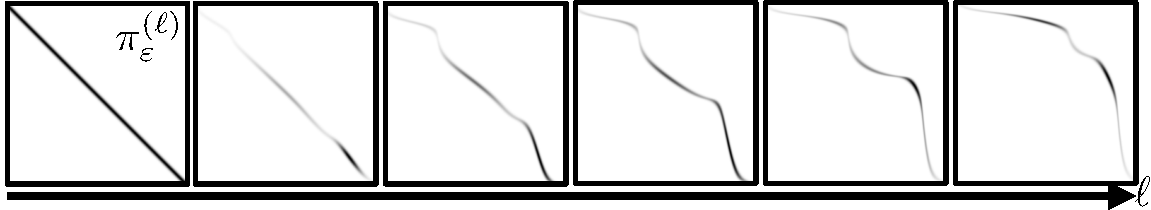
\includegraphics[width=\linewidth]{entropic/sinkhorn-convergence}
\begin{tabular}{c}
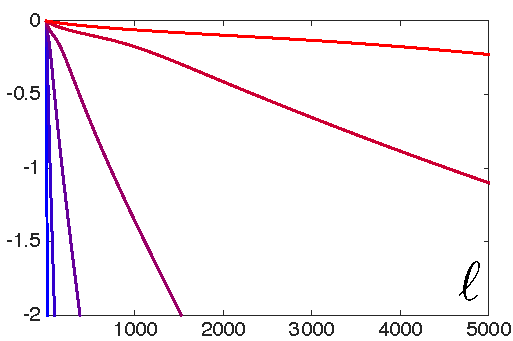
\includegraphics[width=.5\linewidth]{entropic/sinkhorn-rates}\\
{\color{blue}$\varepsilon=10$} \quad {\color[rgb]{0.5,0,0.5}$\varepsilon=0.1$} \quad {\color{red}$\varepsilon=10^{-3}$}
\end{tabular}
\caption{\label{fig-sinkhorn-convergence}
Top: evolution of the coupling $\it{\pi_\varepsilon}=\diag(\it{\uD})\K\diag(\it{\vD})$ computed at iteration $\ell$ of Sinkhorn's iterations, for 1-D densities on $\X=[0,1]$, $c(x,y)=|x-y|^2$, and $\varepsilon=0.1$.
Bottom: impact of $\varepsilon$ the convergence rate of Sinkhorn, as measured in term of marginal constraint violation $\log( \|\it{\pi_\varepsilon} \ones_m - \b \|_1 )$.
}
\end{figure}


%%%%%%%%%%
\begin{rem1}{Overall complexity}\label{rem-complexity-rounding}
	By doing a careful convergence analysis (assuming $n=m$ for the sake of simplicity), \citet{altschuler2017near} showed that by setting $\varepsilon = \frac{4\log(n)}{\tau}$, $O(\norm{\C}_\infty^3 \log(n) \tau^{-3})$ Sinkhorn iterations (with an additional rounding step to compute a valid coupling $\hat \P \in \CouplingsD(\a,\b)$) are enough to ensure that $\dotp{\hat \P}{\C} \leq \MKD_{\C}(\a,\b) + \tau$. This implies that Sinkhorn computes a $\tau$-approximate solution of the unregularized OT problem in $O(n^2\log(n) \tau^{-3})$ operations. The rounding scheme consists in, given two vectors $\uD\in\RR^n,\vD\in\RR^m$ to carry out the following updates (\cite[Alg. 2]{altschuler2017near}):
	$$\begin{aligned}
		\uD'& \eqdef \uD\odot\min\left(\frac{\a}{\uD\odot(\K\vD)},\ones_n\right), 
		\vD' \eqdef \vD\odot \min\left(\frac{\b}{\vD\odot(\transp{\K}\uD')},\ones_n\right), \\
	\Delta_{\a}& \eqdef \a- \uD'\odot (\K \vD'), \Delta_{\b} \eqdef \b- \vD'\odot (\transp{\K} \uD), \\
	\hat\P& \eqdef \diag(\uD')\K\diag(\vD')+\Delta_{\a} \transp{(\Delta_{\b})}/\norm{\Delta_{\a}}_1.
	\end{aligned}$$
	This yields a matrix $\hat\P \in \CouplingsD(\a,\b)$ such that the $1$-norm between $\hat\P$ and $\diag(\uD)\K\diag(\vD)$ is controlled by the marginal violations of $\diag(\uD)\K\diag(\vD)$, namely
	$$ \norm{\hat\P-\diag(\uD)\K\diag(\vD)}_1 \leq \norm{\a-\uD\odot(\K\vD)}_1+\norm{\b-\vD\odot(\transp{\K}\uD)}_1.$$ 
This field remains active, as shown by the recent improvement on the result above by \citet{pmlr-v80-dvurechensky18a}.
\end{rem1}
%%%%%%%%%%

%%%%%%%
\begin{rem}[Numerical stability of Sinkhorn iterations]\label{rem-stability}
As we discuss in Remarks~\ref{rem-global-conv-sinkh} and \ref{rem-local-conv}, the convergence of Sinkhorn's algorithm deteriorates as $\varepsilon\rightarrow 0$. In numerical practice, however, that slowdown is rarely observed in practice for a simpler reason: Sinkhorn's algorithm will often fail to terminate as soon as some of the elements of the kernel $\K$ become too negligible to be stored in memory as positive numbers, and become instead null. This can then result in a matrix product $\K\vD$ or $\transp{\K}\uD$ with ever smaller entries that become null and result in a division by $0$ in the Sinkhorn update of Equation~\eqref{eq-sinkhorn}. Such issues can be partly resolved by carrying out computations on the multipliers $\uD$ and $\vD$ in the log domain. That approach is carefully presented in Remark~\ref{rem-log-sinkh} and is related to a direct resolution of the dual of Problem~\eqref{eq-regularized-discr}.
\end{rem}
%%%%%%%

%%%%%%%
\begin{rem}[Relation with iterative projections]\label{rem-iterative-projection}
Denoting 
\eq{
	\Cc^1_\a \eqdef \enscond{\P}{\P\ones_m=\a}
	\qandq
	\Cc^2_\b \eqdef \enscond{\P}{\transp{\P}\ones_m=\b}
}
the rows and columns constraints, one has $\CouplingsD(\a,\b) = \Cc^1_\a \cap \Cc^2_\b$. One can use Bregman iterative projections~\citep{bregman1967relaxation},
\eql{\label{eq-kl-sinkh-proj}
	\itt{\P} \eqdef \Proj_{\Cc^1_\a}^{\KLD}(\it{\P})
	\qandq
	\ittt{\P} \eqdef \Proj_{\Cc^2_\b}^{\KLD}(\itt{\P}).
}
Since the sets $\Cc^1_\a$ and $\Cc^2_\b$ are affine, these iterations are known to converge to the solution of~\eqref{eq-kl-proj}; see~\citep{bregman1967relaxation}. These iterates are equivalent to Sinkhorn iterations~\eqref{eq-sinkhorn} since defining 
\eq{\label{eq-sink-matrix}\P^{(2\ell)} \eqdef \diag(\it{\uD}) \K \diag(\it{\vD}),}
one has
\begin{align*}
	\P^{(2\ell+1)} &\eqdef \diag(\itt{\uD}) \K \diag(\it{\vD}) \\
	\qandq
	\P^{(2\ell+2)} &\eqdef \diag(\itt{\uD}) \K \diag(\itt{\vD}).
\end{align*}
In practice, however, one should prefer using~\eqref{eq-sinkhorn}, which only requires manipulating scaling vectors and multiplication against a Gibbs kernel, which can often be accelerated (see Remarks~\ref{rem-separable} and~\ref{rem-geod-heat} below). 
\end{rem}
%%%%%%%

%%%%%%%
\begin{rem}[Proximal point algorithm]
In order to approximate a solution of the unregularized ($\epsilon=0$) problem~\eqref{eq-mk-discr}, it is possible to use iteratively the Sinkhorn algorithm, using the so-called proximal point algorithm for the $\KL$ metric. 
%
We denote $F(\P) \eqdef \dotp{\P}{\pi} + \iota_{\CouplingsD(\a,\b)}(\P)$ the unregularized objective function.
%
The proximal point iterations for the $\KLD$ divergence computes a minimizer of $F$, and hence a solution of the unregularized OT problem~\eqref{eq-mk-discr}, by computing iteratively
\eql{\label{eq-prox-point}
	\itt{\P} \eqdef \Prox_{\frac{1}{\epsilon} F}^{\KLD}(\it{\P})
	\eqdef 
	\uargmin{\P \in \RR_+^{n \times m}} \KLD(\P|\it{\P}) + \frac{1}{\epsilon} F(\P)
}
starting from an arbitrary $\init{\P}$ (see also~\eqref{eq-prox-kl}).
%
The proximal point algorithm is the most basic proximal splitting method. 
%
Initially introduced for the Euclidean metric (see, for instance, (\citealt{rockafellar1976monotone})), it extends to any Bregman divergence~\citep{censor1992proximal}, so in particular it can be applied here for the $\KLD$ divergence (see Remark~\ref{rem-bregman}).   
%
The proximal operator is usually not available in closed form, so some form of subiterations are required. 
%
The optimization appearing in~\eqref{eq-prox-point} is very similar to the entropy regularized problem~\eqref{eq-regularized-discr}, with the relative entropy $\KLD(\cdot|\it{\P})$ used in place of the negative entropy $-\HD$. 
%
Proposition~\ref{prop-regularized-primal} and Sinkhorn iterations~\eqref{eq-sinkhorn} carry over to this more general setting when defining the Gibbs kernel as $\K=e^{-\frac{\C}{\epsilon}} \odot \it{\P} = ( e^{-\frac{\C_{i,j}}{\epsilon}} \it{\P}_{i,j} )_{i,j}$.
%
Iterations~\eqref{eq-prox-point} can thus be implemented by running the Sinkhorn algorithm at each iteration.
%
Assuming for simplicity $\init{\P}=\ones_n \ones_m^\top$, these iterations thus have the form 
\begin{align*}
	\itt{P} &= 
		\diag(\it{\uD}) ( e^{-\frac{\C}{\epsilon}} \odot \it{\P} ) \diag(\it{\vD})\\
		&=
		\diag(\it{\uD} \odot \cdots \odot \init{\uD})  
			e^{-\frac{(\ell+1)\C}{\epsilon}} \odot \it{\P} ) 
		\diag(\it{\vD} \odot \cdots \odot \init{\vD}).		
\end{align*}
The proximal point iterates apply therefore iteratively Sinkhorn's algorithm with a kernel $e^{-\frac{\C}{\epsilon/\ell}}$, i.e., with a decaying regularization parameter $\epsilon/\ell$.
%
This method is thus tightly connected to a series of works which combine Sinkhorn with some decaying schedule on the regularization; see, for instance,~\citep{kosowsky1994invisible}. They are efficient in small spacial dimension, when combined with a multigrid strategy to approximate the coupling on an adaptive sparse grid~\citep{schmitzer2016stabilized}.  
\end{rem}
%%%%%%%


%%%%%%%%%
\begin{rem}[Other regularizations]
It is possible to replace the entropic term $-\HD(\P)$ in~\eqref{eq-regularized-discr} by any strictly convex penalty $R(\P)$, as detailed, for instance, in~\citep{dessein2016regularized}. A typical example is the squared $\ell^2$ norm 
\eql{\label{eq-quad-regul}
	R(\P) = \sum_{i,j} \P_{i,j}^2 + \iota_{\RR_+}(\P_{i,j}); 
} 
see~\citep{essid2017quadratically}. 
%
Another example is the family of Tsallis entropies~\citep{muzellec2017tsallis}.
%
Note, however, that if the penalty function is defined even when entries of $\P$ are nonpositive, which is, for instance, the case for a quadratic regularization~\eqref{eq-quad-regul}, then one must add back a nonnegativity constraint $\P \geq 0$, in addition to the marginal constraints $\P\ones_m=\a$ and $\P^\top \ones_n=\b$. Indeed, one can afford to ignore the nonnegativity constraint using entropy because that penalty incorporates a logarithmic term which forces the entries of $\P$ to stay in the positive orthant. This implies that the set of constraints is no longer affine and iterative Bregman projections do not converge anymore to the solution. 
%
A workaround is to use instead~\citeauthor{Dykstra83}'s algorithm~(\citeyear{Dykstra83,Dykstra85}) (see also \citealt{bauschke-lewis}), as detailed in~\citep{2015-benamou-cisc}. This algorithm uses projections according to the Bregman divergence associated to $R$. We refer to Remark~\ref{rem-bregman} for more details regarding Bregman divergences. An issue is that in general these projections cannot be computed explicitly. 
%
For the squared norm~\eqref{eq-quad-regul}, this corresponds to computing the Euclidean projection on $(\Cc^1_\a,\Cc^2_\b)$ (with the extra positivity constraints), which can be solved efficiently using projection algorithms on simplices~\citep{condat2015fast}. The main advantage of the quadratic regularization over entropy is that it produces sparse approximation of the optimal coupling, yet this comes at the expense of a slower algorithm that cannot be parallelized as efficiently as Sinkhorn to compute several optimal transports simultaneously (as discussed in~\S\ref{rem-parallel}). Figure~\ref{fig-quad-regul} contrasts the approximation achieved by entropic and quadratic regularizers. 
\end{rem}
%%%%%%%%%


% G B D H
\newcommand{\myfigRegQuad}[1]{\imgBox{\includegraphics[width=.185\linewidth,trim=65 55 45 40,clip]{quadratic-regul/quadratic-levelsets-#1}}}
\newcommand{\myfigRegEntrop}[1]{\imgBox{\includegraphics[width=.185\linewidth,trim=65 55 45 40,clip]{quadratic-regul/entropy-levelsets-#1}}}

\begin{figure}[h!]
\begin{tabular}{@{}c@{}c@{}c@{}c@{}c@{}}
\myfigRegEntrop{1} &
\myfigRegEntrop{3} &
\myfigRegEntrop{4} &
\myfigRegEntrop{7} &
\myfigRegEntrop{9} \\
{\color[rgb]{.6,.6,0} $\varepsilon=10$} &
{\color[rgb]{.45,.6,.15} $\varepsilon=1$} &
{\color[rgb]{.3,.6,.3} $\varepsilon=0.5 \cdot 10^{-1}$} &
{\color[rgb]{.15,.6,.45} $\varepsilon=10^{-1}$} &
{\color[rgb]{0,.6,.6} $\varepsilon=10^{-3}$} \\
\myfigRegQuad{1} &
\myfigRegQuad{3} &
\myfigRegQuad{4} &
\myfigRegQuad{7} &
\myfigRegQuad{9} \\
{\color[rgb]{.6,.6,0} $\varepsilon=5 \cdot 10^3$} &
{\color[rgb]{.45,.6,.15}$\varepsilon=10^3$} &
{\color[rgb]{.3,.6,.3} $\varepsilon=10^2$} &
{\color[rgb]{.15,.6,.45} $\varepsilon=10$} &
{\color[rgb]{0,.6,.6} $\varepsilon=1$} 
\end{tabular}
\caption{\label{fig-quad-regul}
Comparison of entropic regularization $R=-\HD$ (top row) and quadratic regularization $R=\norm{\cdot}^2+\iota_{\RR_+}$ (bottom row). 
The $(\al,\be)$ marginals are the same as for Figure~\ref{fig-entropic-copula}.
}
\end{figure}



%%%%%%%%%%
\begin{rem1}{Barycentric projection}\label{rem-barycenric-proj}
	Consider again the setting of Remark~\ref{rem:entrop-reg} in which we use entropic regularization to approximate OT between discrete measures. The Kantorovich formulation in \eqref{eq-mk-discr} and its entropic regularization~\eqref{eq-regularized-discr} both yield a coupling $\P \in \CouplingsD(\a,\b)$. In order to define a transportation map $\T : \X \rightarrow \Y$, in the case where $\Y=\RR^\dim$, one can define the so-called barycentric projection map
	\eql{\label{eq-baryproj}
		\T : x_i \in \X \longmapsto \frac{1}{\a_i} \sum_j \P_{i,j} y_j \in \Y,
	}
	where the input measures are discrete of the form~\eqref{eq-pair-discr}. Note that this map is only defined for points $(x_i)_i$ in the support of $\al$. 
	%
	In the case where $\T$ is a permutation matrix (as detailed in Proposition~\ref{prop-matching-kanto}), then $\T$ is equal to a Monge map, and as $\varepsilon \rightarrow 0$, the barycentric projection progressively converges to that map if it is unique.
	%
	For arbitrary (not necessarily discrete) measures, solving~\eqref{eq-mk-generic} or its regularized version~\eqref{eq-entropic-generic} defines a coupling $\pi \in \Couplings(\al,\be)$. Note that this coupling $\pi$ always has a density $\frac{\d\pi(x,y)}{\d\al(x)\d\be(y)}$ with respect to $\al \otimes \be$. A map can thus be retrieved by the formula
	\eql{\label{eq-bary-proj}
		\T : x \in \X \longmapsto \int_\Yy y \frac{\d\pi(x,y)}{\d\al(x)\d\be(y)} \d\be(y).
	}
	In the case where, for $\varepsilon=0$, $\pi$ is supported on the graph of the Monge map (see Remark~\ref{rem-exist-mongemap}), then using $\varepsilon>0$ produces a smooth approximation of this map.
	%	
	Such a barycentric projection is useful to apply the OT Monge map to solve problems in imaging; see Figure~\ref{fig-colors} for an application to color modification. It has also been used to compute approximations of principal geodesics in the space of probability measures endowed with the Wasserstein metric; see~\citep{SeguyCuturi}.
\end{rem1}
%%%%%%%%%



%%%%%%%%%%
\begin{rem1}{Hilbert metric}
As initially explained by~\citep{franklin1989scaling}, the global convergence analysis of Sinkhorn is greatly simplified using the Hilbert projective metric on $\RR_{+,*}^n$ (positive vectors), defined as
\eq{
	\foralls (\uD,\uD') \in (\RR_{+,*}^n)^2, \quad
	\Hilbert(\uD,\uD') \eqdef \log \umax{i,j} \frac{ \uD_i \uD_{j}' }{ \uD_{j} \uD_{i}'  }.
}
It can be shown to be a distance on the projective cone $\RR_{+,*}^n/\sim$, where $\uD \sim \uD'$ means that $\exists r>0, \uD=r\uD'$ (the vectors are equal up to rescaling, hence the name ``projective'').  
%
This means that $\Hilbert$ satisfies the triangular inequality and $\Hilbert(\uD,\uD')=0$ if and only if $\uD \sim \uD'$. 
%
This is a projective version of Hilbert's original distance on bounded open convex sets~\citep{hilbert1895gerade}.
%
The projective cone $\RR_{+,*}^n/\sim$ is a complete metric space for this distance. 
%
By a logarithmic change of variables, the Hilbert metric on the rays of the positive cone is isometric to the variation seminorm (it is a norm between vectors that are defined up to an additive constant)
\eql{\label{eq-hilbert-var}
	\Hilbert(\uD,\uD') = \norm{\log(\uD)-\log(\uD')}_{\text{var}}
}
\eq{
	\qwhereq
	\norm{\fD}_{\text{var}} \eqdef (\max_i \fD_i) - (\min_i \fD_i).
}
%
This variation seminorm is closely related to the $\ell^\infty$ norm since one always has $\norm{\fD}_{\text{var}}  \leq 2 \norm{\fD}_\infty$. If one imposes that $\fD_i=0$ for some fixed $i$, then a converse inequality also holds since $\norm{\fD}_\infty \leq \norm{\fD}_{\text{var}}$. These bounds are especially useful to analyze Sinkhorn convergence (see Remark~\ref{rem-global-conv-sinkh} below), because dual variables $\fD=\log(\uD)$ solving~\eqref{eq-dualsinkhorn-constraints2} are defined up to an additive constant, so that one can impose that $\fD_i=0$ for some $i$.
%
The Hilbert metric was introduced independently by~\citep{birkhoff1957extensions} and~\citep{samelson1957perron}. They proved the following fundamental theorem, which shows that a positive matrix is a strict contraction on the cone of positive vectors.


\begin{thm}\label{thm-birkoff}
	Let $\K \in \RR_{+,*}^{n \times m}$; then for $(\vD,\vD') \in (\RR_{+,*}^m)^2$
	\eq{
		\Hilbert(\K \vD,\K \vD') \leq \la(\K) \Hilbert(\vD,\vD'),
		\text{ where }
		\choice{
			\la(\K) \eqdef \frac{ \sqrt{\eta(\K)}-1 }{ \sqrt{\eta(\K)}+1 } < 1, \\
			\eta(\K) \eqdef \umax{i,j,k,\ell} \frac{ \K_{i,k} \K_{j,\ell} }{ \K_{j,k} \K_{i,\ell} }.
		}
	}
\end{thm}

Figure~\ref{fig-h-m} illustrates this theorem. 
\end{rem1}


\begin{figure}[h!]
\centering
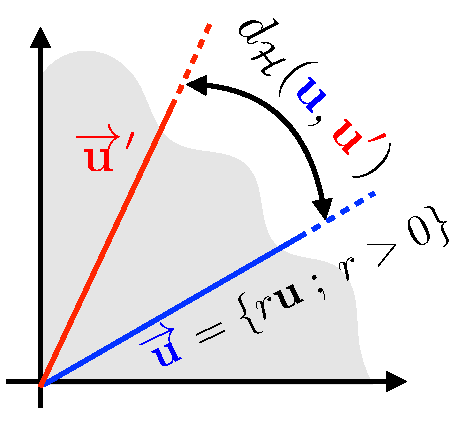
\includegraphics[width=.22\linewidth]{hilbert-metric/hilbert-metric} \qquad
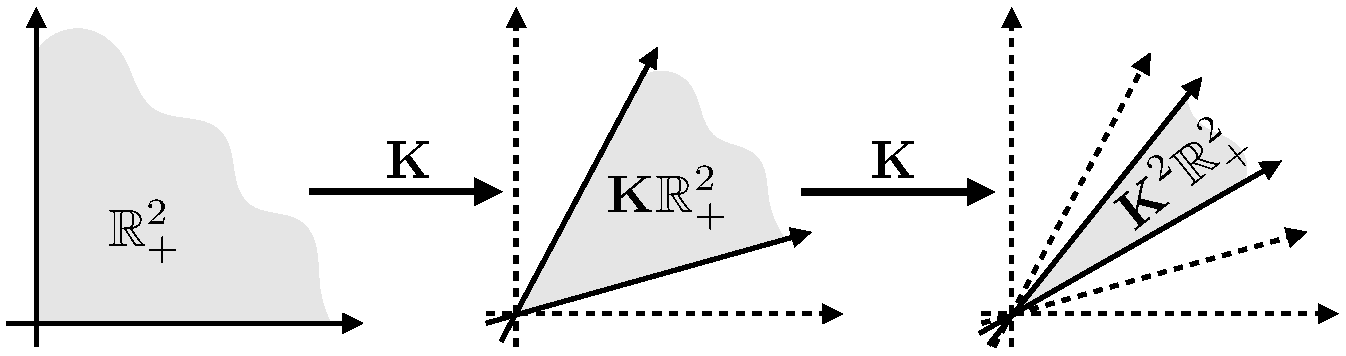
\includegraphics[width=.7\linewidth]{hilbert-metric/cones}\\
\caption{\label{fig-h-m}
Left: the Hilbert metric $\Hilbert$ is a distance over rays in cones (here positive vectors).
Right: visualization of the contraction induced by the iteration of a positive matrix $\K$. 
}
\end{figure}


%%%%%%%%%%
\begin{rem1}{Perron--Frobenius}
A typical application of Theorem~\ref{thm-birkoff} is to provide a quantitative proof of the Perron--Frobenius theorem, which, as explained in Remark~\ref{rem-local-conv}, is linked to a local linearization of Sinkhorn's iterates. A matrix $\K \in \RR_+^{n \times n}$ with $\K^\top \ones_n = \ones_n$ maps $\simplex_n$ into $\simplex_n$. If furthermore $\K>0$, then according to Theorem~\ref{thm-birkoff}, it is strictly contractant for the metric $\Hilbert$, hence there exists a unique invariant probability distribution $p^\star \in \simplex_n$ with $\K p^\star=p^\star$. Furthermore, for any $p_0 \in \simplex_n$, $\Hilbert(\K^\ell p_0,p^\star) \leq \la(\K)^\ell \Hilbert(p_0,p^\star)$, \ie one has linear convergence of the iterates of the matrix toward $p^\star$. This is illustrated in Figure~\ref{fig-perron}.
\end{rem1}
%%%%%%%%%%

\begin{figure}[h!]
\centering
\begin{tabular}{@{}c@{}c@{}c@{\hspace{10mm}}c@{}}
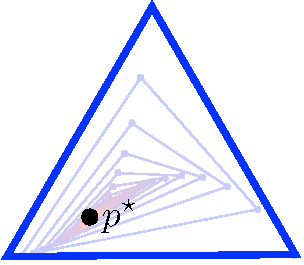
\includegraphics[width=.22\linewidth]{hilbert-metric/simplex-0}&
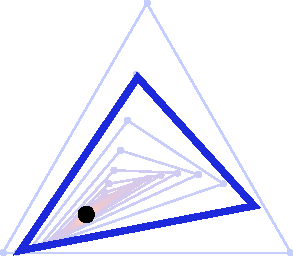
\includegraphics[width=.22\linewidth]{hilbert-metric/simplex-1}&
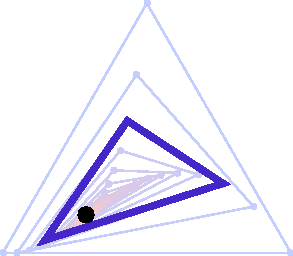
\includegraphics[width=.22\linewidth]{hilbert-metric/simplex-2}&
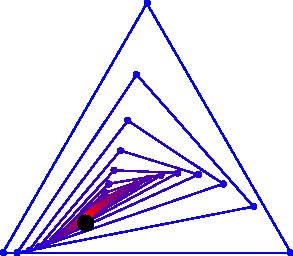
\includegraphics[width=.22\linewidth]{hilbert-metric/simplex-evol}\\
$\simplex_3$ & $\K \simplex_3$ & $\K^2 \simplex_3$ &  $\{ \K^\ell \simplex_3 \}_\ell$
\end{tabular}
\caption{\label{fig-perron}
Evolution of $\K^\ell \simplex_3 \rightarrow \{p^\star\}$ the invariant probability distribution of $\K \in \RR_{+,*}^{3 \times 3}$ with $\K^\top \ones_3=\ones_3$.
}
\end{figure}




%%%%%%%%%%
\begin{rem11}{Global convergence}{rem-global-conv-sinkh}
The following theorem, proved by~\citep{franklin1989scaling}, makes use of Theorem~\ref{thm-birkoff} to show the linear convergence of Sinkhorn's iterations.

\begin{thm}
	One has $(\it{\uD},\it{\vD}) \rightarrow (\uD^\star,\vD^\star)$ and
	\eql{\label{eq-convlin-sinkh}
		\Hilbert(\it{\uD}, \uD^\star) = O(\la(\K)^{2\ell}), \quad
		\Hilbert(\it{\vD}, \vD^\star) = O(\la(\K)^{2\ell}).
	}
	One also has
	\eql{\label{eq-convsinkh-control}
		\begin{split}
		\Hilbert(\it{\uD}, \uD^\star) &\leq \frac{\Hilbert( \it{\P}\ones_m,\a )}{1-\la(\K)^2}, \\
		\Hilbert(\it{\vD}, \vD^\star) &\leq \frac{\Hilbert( \P^{(\ell),\top} \ones_n,\b )}{1-\la(\K)^2},
		\end{split}
	}
	where we denoted $\it{\P} \eqdef \diag(\it{\uD}) \K \diag(\it{\vD})$. Last, one has
	\eql{\label{eq-convlin-sinkh-prim}
		\|\log(\it{\P}) - \log(\P^\star)\|_\infty \leq \Hilbert(\it{\uD}, \uD^\star) + \Hilbert(\it{\vD}, \vD^\star),
	}
	where $\P^\star$ is the unique solution of~\eqref{eq-regularized-discr}. 
\end{thm}

\begin{proof}
	One notices that for any $(\vD,\vD') \in (\RR_{+,*}^m)^2$, one has 
	\eq{	
		\Hilbert(\vD,\vD') = \Hilbert(\vD/\vD',\ones_m) = \Hilbert(\ones_m/\vD,\ones_m/\vD').
	}
	This shows that
	\begin{align*}
		\Hilbert(\itt{\uD},\uD^\star) &= \Hilbert\pa{ \frac{\a}{\K \it{\vD}}, \frac{\a}{\K \vD^\star} } \\
		&= \Hilbert( \K \it{\vD}, \K \vD^\star ) \leq \la(\K) \Hilbert( \it{\vD}, \vD^\star ),
	\end{align*}
	where we used Theorem~\ref{thm-birkoff}. This shows~\eqref{eq-convlin-sinkh}.  One also has, using the triangular inequality,
	\begin{align*}
		\Hilbert(\it{\uD},\uD^\star) &\leq \Hilbert(\itt{\uD},\it{\uD}) + \Hilbert(\itt{\uD},\uD^\star) \\
		&\leq \Hilbert\pa{ \frac{\a}{\K \it{\vD}},\it{\uD} } + \la(\K)^2 \Hilbert(\it{\uD},\uD^\star) \\
		&= \Hilbert\pa{ \a,\it{\uD} \odot  ( \K \it{\vD} ) } + \la(\K)^2 \Hilbert(\it{\uD},\uD^\star), 
	\end{align*}
	which gives the first part of~\eqref{eq-convsinkh-control} since 
	$\it{\uD} \odot  ( \K \it{\vD} ) = \it{\P}\ones_m$ (the second one being similar).
	%
	The proof of~\eqref{eq-convlin-sinkh-prim} follows from~\citep[Lem. 3]{franklin1989scaling}.
\end{proof}
 
The bound~\eqref{eq-convsinkh-control} shows that some error measures on the marginal constraints violation, for instance, $\| \it{\P} \ones_m - \a \|_1$ and $\|\transp{\it{\P}} \ones_n - \b \|_1$, are useful stopping criteria to monitor the convergence.
%
Note that thanks to~\eqref{eq-hilbert-var}, these Hilbert metric rates on the scaling variable $(\it{\uD},\it{\vD})$ give a linear rate on the dual variables $(\it{\fD},\it{\gD}) \eqdef (\varepsilon\log(\it{\uD}),\varepsilon\log(\it{\vD}))$ for the variation norm $\norm{\cdot}_{\text{var}}$.

Figure~\ref{fig-sinkhorn-convergence}, bottom row, highlights this linear rate on the constraint violation and shows how this rate degrades as $\varepsilon\rightarrow 0$. 
%
These results are proved in~\citep{franklin1989scaling} and are tightly connected to nonlinear Perron--Frobenius theory~\citep{lemmens2012nonlinear}. Perron--Frobenius theory corresponds to the linearization of the iterations; see~\eqref{eq-linearized-sinkh}. This convergence analysis is extended by~\citep{linial1998deterministic}, who show that each iteration of Sinkhorn increases the permanence of the scaled coupling matrix. 
\end{rem11}
%%%%%%%%%%



%%%%%%%%%%
\begin{rem1}{Local convergence}\label{rem-local-conv}
The global linear rate~\eqref{eq-convlin-sinkh-prim} is often quite pessimistic, typically in $\X=\Y=\RR^d$ for cases where there exists a Monge map when $\varepsilon=0$ (see Remark~\ref{rem-monge2}). The global rate is in contrast rather sharp for more difficult situations where the cost matrix $\C$ is close to being random, and in these cases, the rate scales exponentially bad with $\varepsilon$, $1-\la(\K) \sim e^{-1/\varepsilon}$.
%
To obtain a finer asymptotic analysis of the convergence (\eg if one is interested in a high-precision solution and performs a large number of iterations), one usually rather studies the local convergence rate. 
%
One can write a Sinkhorn update as iterations of a fixed-point map $\itt{\fD} = \Phi( \it{\fD} )$, where
\eq{
	\Phi \eqdef \Phi_2 \odot \Phi_1
	\qwhereq
	\choice{
		\Phi_1(\fD) = \varepsilon \log \transp{\K} ( e^{\fD/\varepsilon} ) - \log(\b), \\
		\Phi_2(\gD) = \varepsilon \log \K ( e^{\gD/\varepsilon} ) - \log(\a).
	}
}
For optimal $(\fD,\gD)$ solving~\eqref{eq-dual-formulation}, denoting $\P = \diag(e^{\fD/\varepsilon}) \K \diag(e^{\gD/\varepsilon})$ the optimal coupling solving~\eqref{eq-regularized-discr}, one has the following Jacobian:
\eql{\label{eq-linearized-sinkh}
	\partial \Phi(\fD) = \diag(\a)^{-1} \odot \P \odot \diag(\b)^{-1} \odot \transp{\P}.
} 
This Jacobian is a positive matrix with $\partial \Phi(\fD) \ones_n = \ones_n$, and thus by the Perron--Frobenius theorem, it has a single dominant eigenvector $\ones_m$ with associated eigenvalue $1$. Since $\fD$ is defined up to a constant, it is actually the second eigenvalue $1-\kappa<1$ which governs the local linear rate, and this shows that for $\ell$ large enough, 
\eq{
	\|\it{\fD}-\fD \| = O( (1-\kappa)^\ell ).
} 
%
Numerically, in ``simple cases'' (such as when there exists a smooth Monge map when $\varepsilon=0$), this rate scales like $\kappa \sim \varepsilon$. 
%
We refer to~\citep{knight2008sinkhorn} for more details in the bistochastic (assignment) case.
\end{rem1}
%%%%%%%%%%






%%%%%%%%%%%%%%%%%%%%%%%%%%%%%%%%%%%%%%%%%%%%%%%%%%%%%%%%%%%%%%%%%%%%%%%%%%%%%
\section{Speeding Up Sinkhorn's Iterations}

The main computational bottleneck of Sinkhorn's iterations is the vector-matrix multiplication against kernels $\K$ and $\K^\top$, with complexity $O(nm)$ if implemented naively. We now detail several important cases where the complexity can be improved significantly.

%%%%%%%
\begin{rem}[Parallel and GPU friendly computation]\label{rem-parallel} The simplicity of Sinkhorn's algorithm yields an extremely efficient approach to compute simultaneously several regularized Wasserstein distances between pairs of histograms. 
Let $N$ be an integer, $\a_1,\ldots,\a_N$ be histograms in $\simplex_n$, and $\b_1,\ldots,\b_N$ be histograms in $\Sigma_m$. 
We seek to compute all $N$ approximate distances $\MKD_\C^\varepsilon(\a_1,\b_1),\dots,\MKD_\C^\varepsilon(\a_N,\b_N)$. 
In that case, writing $\A=[\a_1,\dots,\a_N]$ and $\B=[\b_1,\dots,\b_N]$ for the $n\times N$ and $m\times N$ matrices storing all histograms, one can notice that all Sinkhorn iterations for all these $N$ pairs can be carried out in parallel, by setting, for instance,
\eql{\label{eq-sinkhorn-par}	
	\itt{\UD} \eqdef \frac{\A}{\K \it{\VD}}
	\qandq
	\itt{\VD} \eqdef \frac{\B}{\transp{\K}\itt{\UD}},
}
initialized with $\init{\VD} = \ones_{m \times N}$. Here $\frac{\cdot}{\cdot}$ corresponds to the entrywise division of matrices.
One can further check that upon convergence of $\VD$ and $\UD$, the (row) vector of regularized distances simplifies to
$$ \transp{\ones_n} (    \UD\odot \log \UD \odot (   (\K\odot \C) \VD) +  \UD\odot(   (\K\odot \C)(\VD\odot \log \VD)    ) ) \in\RR^{N}.$$
Note that the basic Sinkhorn iterations described in Equation~\eqref{eq-sinkhorn} are intrinsically GPU friendly, since they only consist in matrix-vector products, and this was exploited, for instance, to solve matching problems in~\citet{slomp2011gpu}). However, the matrix-matrix operations presented in Equation~\eqref{eq-sinkhorn-par} present even better opportunities for parallelism, which explains the success of Sinkhorn's algorithm to compute OT distances between histograms at large scale.
\end{rem}
%%%%%%%

%%%%%%%%%
\begin{rem}[Speed-up for separable kernels]\label{rem-separable} We consider in this section an important particular case for which the complexity of each Sinkhorn iteration can be significantly reduced. That particular case happens when each index $i$ and $j$ considered in the cost-matrix can be described as a $d$-uple taken in the cartesian product of $d$ finite sets $\range{n_1},\dots,\range{n_d}$,
$$i=(i_k)_{k=1}^d, j=(j_k)_{k=1}^d \in \range{n_1}\times\dots\times\range{n_d}.$$
In that setting, if the cost $\C_{ij}$ between indices $i$ and $j$ is additive along these sub-indices, namely if there exists $d$ matrices $\C^1,\dots,\C^d$, each of respective size $n_1\times n_,\dots,n_d\times n_d$, such that
$$\C_{ij} = \sum_{k=1}^d \C^k_{i_k,j_k},$$
then one obtains as a direct consequence that the kernel appearing in the Sinkhorn iterations has a separable multiplicative structure,
\eql{\label{eq-speedup-separable}
\K_{i,j} = \prod_{k=1}^d \K^k_{i_k,j_k}.
}
Such a separable multiplicative structure allows for a very fast (exact) evaluation of $\K \uD$. Indeed, instead of instantiating $\K$ as a matrix of size $n\times n$, which would have a prohibitive size since $n=\prod_k n_k$ is usually exponential in the dimension $d$, one can instead recover $\K\uD$ by simply applying $\K^k$ along each ``slice'' of $\uD$. If $n=m$, the complexity reduces to $O(n^{1+1/d})$ in place of $O(n^2)$.
%

An important example of this speed-up arises when $\Xx=\Yy=[0,1]^d$; the ground cost is the $q$-th power of the $q$-norm, $$\c(x,y)=\norm{x-y}^q_q=\sum_{i=1}^d |x_i-y_i|^q, \; q>0;$$ and the space is discretized using a regular grid in which only points $x_i = (i_1/n_1,\ldots,i_d/n_d)$ for $i=(i_1,\dots,i_d)\in\range{n_1}\times \dots\times\range{n_d}$ are considered. In that case a multiplication by $\K$ can be carried out more efficiently by applying each 1-D $n_k\times n_k$ convolution matrix $$\K^k = \begin{bmatrix}\exp(-\left|\frac{r-s}{n_k}\right|^q/ \varepsilon)\end{bmatrix}_{1 \leq r,s\leq n_k}$$ to $\uD$ reshaped as a tensor whose first dimension has been permuted to match the $k$-th set of indices.
%
For instance, if $d=2$ (planar case) and $q=2$ (2-Wasserstein, resulting in Gaussian convolutions), histograms $\a$ and as a consequence Sinkhorn multipliers $\uD$ can be instantiated as $n_1\times n_2$ matrices. We write $\mathbf{U}$ to underline the fact that the multiplier $\uD$ is reshaped as a $n_1\times n_2$ matrix, rather than a vector of length $n_1n_2$. Then, computing $\K\uD$, which would naively require $(n_1 n_2)^2$ operations with a naive implementation, can be obtained by applying two 1-D convolutions separately, as $$(\K^2(\K^1 \mathbf{U})^T)^T=\K^1\mathbf{U}\K^2,$$ to recover a $n_1\times n_2$ matrix in $(n_1^2)n_2+n_1(n_2^2)$ operations instead of $n_1^2n_2^2$ operations. Note that this example agrees with the exponent $(1+1/d)$ given above. With larger $d$, one needs to apply these very same 1-D convolutions to each slice of $\uD$ (reshaped as a tensor of suitable size) an operation which is extremely efficient on GPUs.
%

This important observations underlies many of the practical successes found when applying optimal transport to shape data in 2-D and 3-D, as highlighted in~\citep{2015-solomon-siggraph,2016-bonneel-barycoord}, in which distributions supported on grids of sizes as large as $200^3=8 \times 10^6$ are handled.
\end{rem}
%%%%%%%%%

%%%%%%%%%
\begin{rem}[Approximated convolutions]\label{rem-convol-sinkh}
The main computational bottleneck of Sinkhorn's iterations~\eqref{eq-sinkhorn} lies in the multiplication of a vector by $\K$ or by its adjoint. Besides using separability~\eqref{eq-speedup-separable}, it is also possible to exploit other special structures in the kernel. The simplest case is for translation invariant kernels $\K_{i,j} = k_{i-j}$, which is typically the case when discretizing the measure on a fixed uniform grid in Euclidean space $\X=\RR^\dim$. Then $\K \vD = k \star \vD$ is a convolution, and there are several algorithms to approximate the convolution in nearly linear time. 
%
The most usual one is by Fourier transform $\Ff$, assuming for simplicity periodic boundary conditions, because $\Ff(k \star \vD)=\Ff(k) \odot \Ff(\vD)$. This leads, however, to unstable computations and is often unacceptable for small $\varepsilon$.
%
Another popular way to speed up computation is by approximating the convolution using a succession of autoregressive filters, using, for instance, the Deriche filtering method~\citet{deriche1993recursively}. We refer to~\citep{getreuer2013survey} for a comparison of various fast filtering methods.
\end{rem}
%%%%%%%%%

%%%%%%%%%
\begin{rem}[Geodesic in heat approximation]\label{rem-geod-heat}
For nonplanar domains, the kernel $\K$ is not a convolution, but in the case where the cost is $\C_{i,j}=d_\Mm(x_i,y_j)^p$ where $d_\Mm$ is a geodesic distance on a surface $\Mm$ (or a more general manifold), it is also possible to perform fast approximations of the application of $\K=e^{-\frac{d_\Mm}{\varepsilon}}$ to a vector. Indeed, \citeauthor{varadhan-1967}'s formulas~\citeyearpar{varadhan-1967} assert that this kernel is close to the Laplacian kernel (for $p=1$) and the heat kernel (for $p=2$). 
%
The first formula of Varadhan states
\eql{\label{eq-varadhan-1}
	-\frac{\sqrt{t}}{2} \log( \Pp_t(x,y) ) = d_\Mm(x,y) + o(t)
	\qwhereq
	\Pp_t \eqdef (\Id - t\De_{\Mm})^{-1},
}
where $\De_{\Mm}$ is the Laplace--Beltrami operator associated to the manifold $\Mm$ (which is negative semidefinite), so that 
$\Pp_t$ is an integral kernel and $g = \int_\Mm \Pp_t(x,y) f(y) \d y$ is the solution of $g - t \De_{\Mm} g = f$. 
%
The second formula of Varadhan states
\eql{\label{eq-varadhan-2}
	\sqrt{ -4 t \log( \Hh_t(x,y) ) } = d_\Mm(x,y) + o(t),
}
where  $\Hh_t$ is the integral kernel defined so that $g_t = \int_\Mm \Hh_t(x,y) f(y) \d y$ is the solution at time $t$ of the heat equation
\eq{
	\frac{\partial g_t(x)}{\partial t} = (\Delta_\Mm g_t)(x).
}
The convergence in these formulas~\eqref{eq-varadhan-1} and~\eqref{eq-varadhan-2} is uniform on compact manifolds.
%
Numerically, the domain $\Mm$ is discretized (for instance, using finite elements) and $\De_\Mm$ is approximated by a discrete Laplacian matrix $L$. A typical example is when using piecewise linear finite elements, so that $L$ is the celebrated cotangent Laplacian (see~\citep{botsch-2010} for a detailed account for this construction).
%
These formulas can be used to approximate efficiently the multiplication by the Gibbs kernel $\K_{i,j}=e^{-\frac{d(x_i,y_j)^p}{\varepsilon}}$.
%
Equation~\eqref{eq-varadhan-1} suggests, for the case $p=1$, to use $\varepsilon=\frac{\sqrt{t}}{2}$ and to replace the multiplication by $\K$ by the multiplication by $(\Id-t L)^{-1}$, which necessitates the resolution of a positive symmetric linear system.
%
Equation~\eqref{eq-varadhan-2}, coupled with $R$ steps of implicit Euler for the stable resolution of the heat flow, suggests for $p=2$ to trade the multiplication by $\K$ by the multiplication by $(\Id-\frac{t}{R} L)^{-R}$ for $4 t=\varepsilon$, which in turn necessitates $R$ resolutions of linear systems. Fortunately, since these linear systems are supposed to be solved at each Sinkhorn iteration, one can solve them efficiently by precomputing a sparse Cholesky factorization. By performing a reordering of the rows and columns of the matrix~\citep{george1989evolution}, one obtains a nearly linear sparsity for 2-D manifolds and thus each Sinkhorn iteration has linear complexity (the performance degrades with the dimension of the manifold). 
%
The use of Varadhan's formula to approximate geodesic distances was initially proposed in~\citep{Crane2013} and its use in conjunction with Sinkhorn iterations in~\citep{2015-solomon-siggraph}.
%
\todoK{Maybe add some pedagological figure illustrating the method.}
\end{rem}
%%%%%%%%%


%%%%%%%%%%
\begin{rem}[Extrapolation acceleration]
	Since the Sinkhorn algorithm is a fixed-point algorithm (as shown in Remark~\ref{rem-local-conv}), one can use standard linear or even nonlinear extrapolation schemes to enhance the conditioning of the fixed-point mapping near the solution, and improve the linear convergence rate. 
	%
	This is similar to the successive overrelaxation  method (see, for instance,~\citep{hadjidimos2000successive}), so that the local linear rate of convergence is improved from $O((1-\kappa)^\ell)$ to $O((1-\sqrt{\kappa})^\ell)$ for some $\kappa>0$ (see Remark~\ref{rem-local-conv}). 
	%
	We refer to~\citep{2016-peyre-qot} for more details\todoK{citer papier recent Lenaic}.
\end{rem}
%%%%%%%%%%



%%%%%%%%%%%%%%%%%%%%%%%%%%%%%%%%%%%%%%%%%%%%
\section{Stability and Log-Domain Computations}

As briefly mentioned in Remark~\ref{rem-stability}, the Sinkhorn algorithm suffers from numerical overflow when the regularization parameter $\epsilon$ is small compared to the entries of the cost matrix $\C$. This concern can be alleviated to some extent by carrying out computations in the log domain. The relevance of this approach is made more clear by considering the dual problem associated to~\eqref{eq-regularized-discr}, in which these log-domain computations arise naturally.

\begin{prop}
One has
\eql{\label{eq-dual-formulation}
	\MKD_\C^\varepsilon(\a,\b) = \umax{\fD \in \RR^n,\gD \in \RR^m}
		 \dotp{\fD}{\a} + \dotp{\gD}{\b} 
		% - \varepsilon\sum_{i,j} e^{ \frac{\fD_i+\gD_j-\C_{i,j}}{\varepsilon} }.
		- \varepsilon \dotp{e^{\fD/\varepsilon} }{ \K e^{\gD/\varepsilon}}.
} 
%
The optimal $(\fD,\gD)$ are linked to scalings $(\uD,\vD)$ appearing in~\eqref{eq-scaling-form} through 
\eql{\label{eq-entropy-pd}
	(\uD,\vD)=(e^{\fD/\varepsilon},e^{\gD/\varepsilon}).
}
\end{prop}

\begin{proof}
We start from the end of the proof of Proposition~\ref{prop-regularized-primal}, which links the optimal primal solution $\P$ and dual multipliers $\fD$ and $\gD$ for the marginal constraints as 
\eq{
	\label{eq-prim-dual-ent}\P_{i,j}=e^{\fD_i/\varepsilon}e^{-\C_{i,j}/\varepsilon}e^{\gD_j/\varepsilon}.
} 
Substituting in the Lagrangian $\Lag(\P,\fD,\gD)$ of Equation~\eqref{eq-sinkhorn-lagrangian} the optimal $\P$ as a function of $\fD$ and $\gD$, we obtain that the Lagrange dual function equals
\eql{\label{eq-lagrange-dual-naive}
	\fD,\gD \mapsto \dotp{e^{\fD/\varepsilon}}{\left(\K\odot \C\right)e^{\gD/\varepsilon}} - \varepsilon \HD(\diag(e^{\fD/\varepsilon}) \K \diag(e^{\gD/\varepsilon})).
}
The neg-entropy of $\P$ scaled by $\varepsilon$, namely $\varepsilon \dotp{\P}{\log \P - \ones_{n\times m}}$, can be stated explicitly as a function of $\fD,\gD, \C$,
\begin{align*}
&\dotp{\diag(e^{\fD/\varepsilon}) \K \diag(e^{\gD/\varepsilon})}{\fD\transp{\ones_m}+\ones_n\transp{\gD}-\C-\varepsilon\ones_{n\times m}}\\
&= -\dotp{e^{\fD/\varepsilon}}{\left(\K\odot \C\right)e^{\gD/\varepsilon}} + \dotp{\fD}{\a}+ \dotp{\gD}{\b}-\varepsilon \dotp{e^{\fD/\varepsilon}}{\K e^{\gD/\varepsilon}};
\end{align*}
therefore, the first term in~\eqref{eq-lagrange-dual-naive} cancels out with the first term in the entropy above. The remaining terms are those appearing in~\eqref{eq-dual-formulation}.
\end{proof}


	
%%%%%%%%%%
\begin{rem}[Sinkhorn as a block coordinate ascent on the dual problem]\label{rem-sinkh-block}
A simple approach to solving the unconstrained maximization problem~\eqref{eq-dual-formulation} is to use an exact \emph{block coordinate ascent} strategy, namely to update alternatively $\fD$ and $\gD$ to cancel the respective gradients in these variables of the objective of \eqref{eq-dual-formulation}. Indeed, one can notice after a few elementary computations that, writing $Q(\fD,\gD)$ for the objective of~\eqref{eq-dual-formulation},
\begin{align}
	\label{eq-dualupadate-sinkh-1}\nabla|_\fD\, Q(\fD,\gD) &=  \a - e^{\fD/\varepsilon}\odot \left(\K e^{\gD/\varepsilon}\right),\\
	\label{eq-dualupadate-sinkh-2}\nabla|_\gD\, Q(\fD,\gD) &=  \b - e^{\gD/\varepsilon}\odot \left(\transp{\K} e^{\fD/\varepsilon}\right).
\end{align}
Block coordinate ascent can therefore be implemented in a closed form by applying successively the following updates, starting from any arbitrary $\init{\gD}$, for $l\geq 0$:
\begin{align}
	\label{eq-slse-sinkh-1}\itt{\fD} &= \varepsilon \log \a -\varepsilon\log\left(\K e^{\it{\gD}/\varepsilon}\right), \\
	\label{eq-slse-sinkh-2}\itt{\gD} &= \varepsilon \log \b- \varepsilon\log\left(\transp{\K} e^{\itt{\fD}/\varepsilon}\right).
\end{align}
Such iterations are mathematically equivalent to the Sinkhorn iterations~\eqref{eq-sinkhorn} when considering the primal-dual relations highlighted in~\eqref{eq-entropy-pd}. Indeed, we recover that at any iteration
\eq{
	(\it{\fD},\it{\gD}) = \varepsilon ( \log(\it{\uD}), \log(\it{\vD}) ). 
}
\end{rem}
%%%%%%%%%%

%%%%%%%%%%
\begin{rem}[Soft-min rewriting]
Iterations~\eqref{eq-slse-sinkh-1} and~\eqref{eq-slse-sinkh-2} can be given an alternative interpretation, using the following notation. Given a vector $\z$ of real numbers we write $\smine\z$ for the \emph{soft-minimum} of its coordinates, namely
\eql{\label{eq-defn-softmin}
	\smine\z= -\varepsilon \log \sum_i e^{-\z_i/\varepsilon}.
}
Note that $\smine(\z)$ converges to $\min\,\z$ for any vector $\z$ as $\varepsilon\rightarrow 0$. Indeed, $\smine$ can be interpreted as a differentiable approximation of the $\min$ function, as shown in Figure~\ref{fig-softmin}. 

\begin{figure}[h!]
\centering
\begin{tabular}{@{}c@{\hspace{1mm}}c@{\hspace{1mm}}c@{\hspace{1mm}}c@{\hspace{1mm}}c@{}}

\includegraphics[width=.19\linewidth]{soft-min/lse-1}&
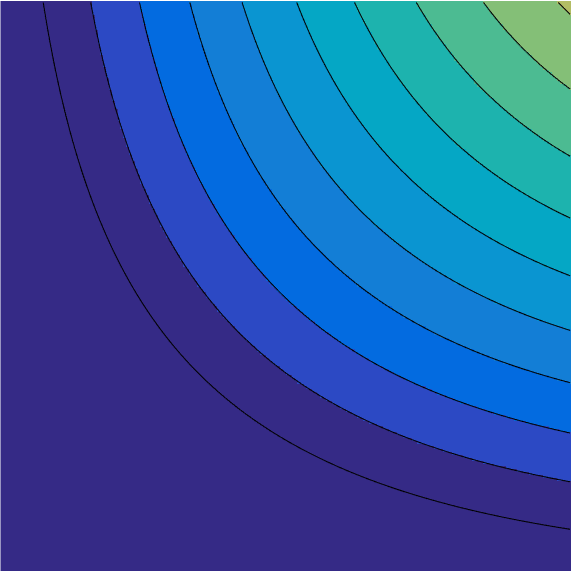
\includegraphics[width=.19\linewidth]{soft-min/lse-05}&
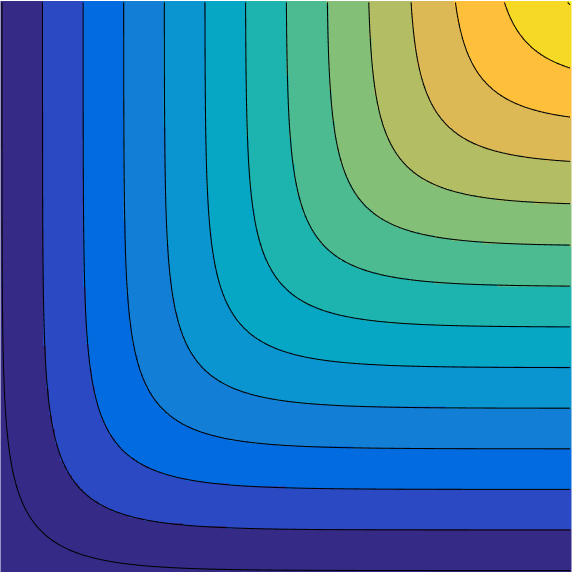
\includegraphics[width=.19\linewidth]{soft-min/lse-01}&
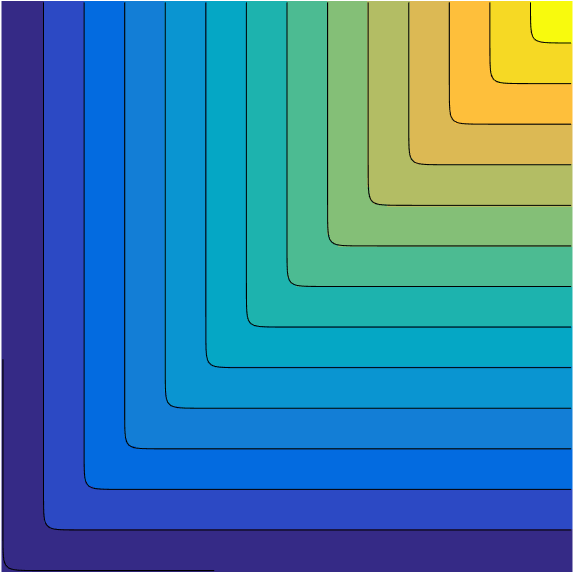
\includegraphics[width=.19\linewidth]{soft-min/lse-001}&
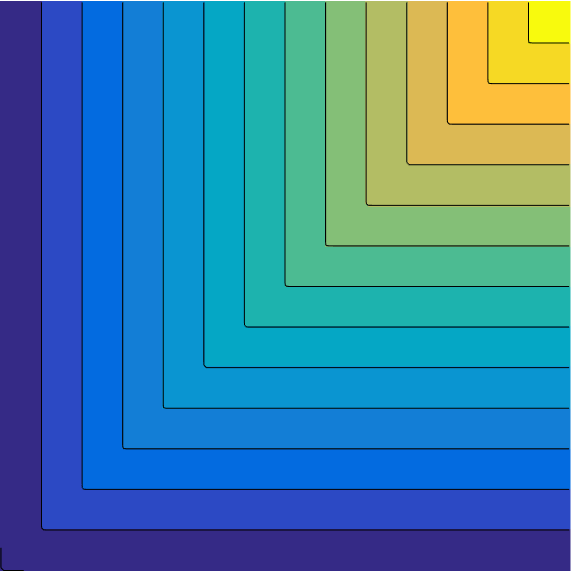
\includegraphics[width=.19\linewidth]{soft-min/lse-0001} \\
$\varepsilon=1$ &
$\varepsilon=0.5$ &
$\varepsilon=10^{-1}$ &
$\varepsilon=10^{-2}$ &
$\varepsilon=10^{-3}$ 
\end{tabular}
\caption{\label{fig-softmin}
Display of the function $\smine(\z)$ in 2-D, $\z \in \RR^2$, for varying~$\varepsilon$.
}
\end{figure}

Using this notation, Equations~\eqref{eq-slse-sinkh-1} and~\eqref{eq-slse-sinkh-2} can be rewritten
\begin{align}
\label{eq-slse-smin-1}(\itt{\fD})_i &= \smine\, (\C_{ij}-\it{\gD}_j)_j + \varepsilon \log \a_i, \\
\label{eq-slse-smin-2}(\itt{\gD})_j &= \smine\, (\C_{ij}-\it{\fD}_i)_i + \varepsilon \log \b_j.
\end{align}
Here the term $\smine\, (\C_{ij}-\it{\gD}_j)_j$ denotes the soft-minimum of all values of the $j$th column of matrix $(\C-\ones_n (\it{\gD})^\top )$. To simplify notations, we introduce an operator that takes a matrix as input and outputs now a column vector of the soft-minimum values of its columns or rows. Namely, for any matrix $A\in\RR^{n\times m}$, we define
\begin{align*}
	\SMINEr(\A) \eqdef \pa{\smine \pa{\A_{i,j}}_j}_i\in\RR^n,\\ 
	\SMINEc(\A) \eqdef \pa{\smine \pa{\A_{i,j}}_i}_j\in\RR^m.
\end{align*}
Note that these operations are equivalent to the entropic $\c$-transform introduced in~\S\ref{sec-semi-discr-entropy} (see in particular~\eqref{eq-sinkh-c-transf}).
%
Using this notation, Sinkhorn's iterates read
\begin{align}
	\label{eq-lse-dual-1}\itt{\fD} &= \SMINEr\, (\C-\ones_n\transp{\it{\gD}}) + \varepsilon \log \a, \\
	\label{eq-lse-dual-2}\itt{\gD} &= \SMINEc\, (\C-\it{\fD}\transp{\ones_m})  + \varepsilon \log \b.
\end{align}
Note that as $\varepsilon \rightarrow 0$, $\smine$ converges to $\min$, but the iterations do not converge anymore in the limit $\varepsilon=0$, because alternate minimization does not converge for constrained problems, which is the case for the unregularized dual~\eqref{eq-dual}.
\end{rem}
%%%%%%%%%%



%%%%%%%%%%
\begin{rem}[Log-domain Sinkhorn]\label{rem-log-sinkh}
While mathematically equivalent to the Sinkhorn updates~\eqref{eq-sinkhorn}, iterations~\eqref{eq-slse-smin-1} and~\eqref{eq-slse-smin-2} suggest using the \emph{log-sum-exp} stabilization trick to avoid underflow for small values of $\varepsilon$. Writing $\underbar{z}=\min \z$, that trick suggests evaluating $\smine \z$ as
\eql{\label{eq-log-domain-min}
	\smine \z = \underbar{z} -\varepsilon \log \sum_i e^{-(\z_i-\underbar{z})/\varepsilon}.
}
Instead of substracting $\underbar{z}$ to stabilize the log-domain iterations as in~\eqref{eq-log-domain-min}, one can actually substract the previously computed scalings. 
This leads to the stabilized iteration
\begin{align}
	\label{eq-lse-sinkh-1}\itt{\fD} &= \SMINEr( \logP(\it{\fD},\it{\gD}))  + \it{\fD} + \varepsilon\log(\a), \\
	\label{eq-lse-sinkh-2}\itt{\gD} &= \SMINEc( \logP(\itt{\fD},\it{\gD})) + \it{\gD} + \varepsilon \log(\b), 
\end{align}
where we defined
\eq{
	\logP(\fD,\gD) = \pa{\C_{i,j} - \fD_i - \gD_j}_{i,j}.
}
% The log-sum-exp operators are defined as
% \begin{align*}
% 	\foralls i \in \range{n}, \quad \LSE_1(\logP)_i &= \varepsilon \log \sum_j \exp( \logP_{i,j} ), \\
% 	\foralls j \in \range{m}, \quad \LSE_2(\logP)_j &= \varepsilon \log \sum_i \exp( \logP_{i,j} ).
% \end{align*}
In contrast to the original iterations~\eqref{eq-sinkhorn}, these log-domain iterations~\eqref{eq-lse-sinkh-1} and~\eqref{eq-lse-sinkh-2} are stable for arbitrary $\varepsilon>0$,
because the quantity $\logP(\fD,\gD)$ stays bounded during the iterations. 
The downside is that it requires $nm$ computations of $\exp$ at each step. 
Computing a $\SMINEr$ or $\SMINEc$ is typically substantially slower than matrix multiplications and requires computing line by line soft-minima of matrices $\logP$. There is therefore no efficient way to parallelize the application of Sinkhorn maps for several marginals simultaneously.
%
In Euclidean domains of small dimension, it is possible to develop efficient multiscale solvers with a decaying $\varepsilon$ strategy to significantly speed up the computation using sparse grids~\citep{schmitzer2016stabilized}.
\end{rem}
%%%%%%%%%%




%%%%%%%%%%
\begin{rem2}{Dual for generic measures}
For generic and not necessarily discrete input measures $(\al,\be)$, the dual problem~\eqref{eq-dual-formulation} reads
\eql{\label{eq-dual-entropic}
	\usup{(\f,\g) \in \Cc(\X)\times\Cc(\Y)} \int_\X \f \d\al + \int_\Y \g \d\be 
		 - \varepsilon \int_{\X\times\Y} e^{ \frac{-c(x,y)+f(x)+g(y)}{\varepsilon} } \d\al(x)\d\be(y).
}
This corresponds to a smoothing of the constraint $\Potentials(\c)$ appearing in the original problem~\eqref{eq-dual-generic}, which is retrieved in the limit $\varepsilon \rightarrow 0$.
%
Proving existence (\ie the sup is actually a max) of these Kantorovich potentials $(\f,\g)$ in the case of entropic transport is less easy than for classical OT, because one cannot use the $c$-transform and potentials are not automatically Lipschitz. Proof of existence can be done using the convergence of Sinkhorn iterations; see~\citep{2016-chizat-sinkhorn} for more details. 
\end{rem2}
%%%%%%%%%%




%%%%%%%
\begin{rem2}{Unconstrained entropic dual}
As in Remark~\ref{rem-uncons-dual}, in the case $\int_\X \d\mu=\int_\Y\d\nu = 1$, one can consider an  alternative dual formulation
\eql{\label{eq-dual-entropic-alt}
	\usup{(\f,\g) \in \Cc(\X)\times\Cc(\Y)} \int_\X \f \d\al + \int_\Y \g \d\be 
		+ \smine( c - f \oplus g ),
}
which achieves the same optimal value as~\eqref{eq-dual-entropic}.
%
Similarly to~\eqref{eq-defn-softmin}, the soft-minimum (here on $\X \times \Y$) is defined as
\eq{
	\foralls S \in \Cc(\X\times\Y), \quad
	\smine S \eqdef 
	- \varepsilon \int_{\X\times\Y} e^{ \frac{-S(x,y)}{\varepsilon} } \d\al(x)\d\be(y)
}
(note that it depends on $(\al,\be)$).
% 
As $\epsilon \rightarrow 0$, $\smine \rightarrow \min$, as used in the unregularized and unconstrained formulation~\eqref{eq-dual-uncons}.
%
Note that while both~\eqref{eq-dual-entropic} and~\eqref{eq-dual-entropic-alt} are unconstrained problems, 
a chief advantage of~\eqref{eq-dual-entropic-alt} is that it is better conditioned, 
in the sense that the Hessian of the functional is uniformly bounded by $\epsilon$. 
Another way to obtain such a conditioning improvement is to consider semidual problems; 
see \S\ref{sec-semi-discr-entropy} and in particular Remark~\ref{rem-second-order-smoothness}.
% 
A disadvantage of this alternative dual formulation is that the presence of a log prevents the use of stochastic optimization methods as detailed in \S\ref{sec-sgd}; see in particular Remark~\ref{rem-sgd-cont-cont}.
\end{rem2}
%%%%%%%

%%%%%%%%%%%%%%%%%%%%%%%%%%%%%%%%%%%%%%%%%%%%%%%%%%%%%%%%%%%%%%%%%%%%%%%%%%
\section{Regularized Approximations of the Optimal Transport Cost}
\label{sec-regularized-cost}

The entropic dual~\eqref{eq-dual-formulation} is a smooth unconstrained concave maximization problem, which approximates the original Kantorovich dual~\eqref{eq-dual}, as detailed in the following proposition. \todoK{explain soft indicator constraint, transition to result below.}

\begin{prop}\label{prop-feasibility-dual}
Any pair of optimal solutions $(\fD^\star,\gD^\star)$ to~\eqref{eq-dual-formulation} are such that $(\fD^\star,\gD^\star) \in \PotentialsD(\C)$, the set of feasible Kantorovich potentials defined in~\eqref{eq-feasible-potential}. As a consequence, we have that for any $\varepsilon$,
\eq{
	\dotp{\fD^\star}{\a} + \dotp{\gD^\star}{\b} \leq  \MKD_\C(\a,\b).
}
\end{prop}
\begin{proof}
	Primal-dual optimality conditions in~\eqref{eq-prim-dual-ent} with the constraint that $\P$ is a probability and therefore $\P_{i,j}\leq 1$ for all $i,j$ yields that $\exp(-(\fD^\star_i+\gD^\star_j-\C_{i,j})/\varepsilon)\leq 1$ and therefore that $\fD^\star_i+\gD^\star_j\leq\C_{i,j}$.
\end{proof}

A chief advantage of the regularized transportation cost $\MKD_\C^\varepsilon$ defined in~\eqref{eq-regularized-discr} is that it is smooth and convex, which makes it a perfect fit for integrating as a loss function in variational problems (see Chapter~\ref{c-variational}).

\begin{prop}\label{prop-convexity-dual}
$\MKD_\C^\varepsilon(\a,\b)$ is a jointly convex function of $\a$ and $\b$ for $\epsilon\geq 0$. When $\epsilon>0$, its gradient is equal to
\eq{
	\nabla\MKD_\C^\varepsilon(\a,\b)= \begin{bmatrix} \fD^\star \\ \gD^\star \end{bmatrix},
}
where $\fD^\star$ and $\gD^\star$ are the optimal solutions of Equation~\eqref{eq-dual-formulation} chosen so that their coordinates sum to 0.
\end{prop}

\todoK{
\begin{proof}
	\todo{TODO}
\end{proof}
}


In \citep{CuturiSinkhorn}, lower and upper bounds to approximate the Wasserstein distance between two histograms were proposed. These bounds consist in evaluating the primal and dual objectives at the solutions provided by the Sinkhorn algorithm.

\begin{defn}[Sinkhorn divergences]
	Let $\fD^\star$ and $\gD^\star$ be optimal solutions to~\eqref{eq-dual-formulation} and $\P^\star$ be the solution to~\eqref{eq-regularized-discr}. The Wasserstein distance is approximated using the following primal and dual Sinkhorn divergences:
\begin{align*}
	\SINKHORNP_\C^\varepsilon(\a,\b)& \eqdef \dotp{\C}{\P^\star} =  \dotp{e^{\frac{\fD^\star}{\varepsilon}}}{(\K\odot \C)e^{\frac{\gD^\star}{\varepsilon}}}, \\
	\SINKHORND_\C^\varepsilon(\a,\b) & \eqdef \dotp{\fD^\star}{\a} + \dotp{\gD^\star}{\b},
\end{align*}
where $\odot$ stands for the elementwise product of matrices, 
\end{defn}

\begin{prop}\label{prop-sinkhorn-div}
The following relationship holds:
\eq{
	\SINKHORND_\C^\varepsilon(\a,\b)\leq \MKD_\C^\varepsilon(\a,\b) \leq \SINKHORNP_\C^\varepsilon(\a,\b).
}
Furthermore
\eql{\label{eq-sinkh-div-gap}
	\SINKHORNP_\C^\varepsilon(\a,\b) - \SINKHORND_\C^\varepsilon(\a,\b) = \varepsilon ( \HD(\P^\star)+1 ) .
}
\end{prop}
\begin{proof}
Equation~\eqref{eq-sinkh-div-gap} is obtained by writing that the primal and dual problems have the same values at the optima (see~\eqref{eq-dual-formulation}), and hence
\eq{
	\MKD_\C^\varepsilon(\a,\b) = \SINKHORNP_\C^\varepsilon(\a,\b) - \varepsilon \HD(\P^\star) = 
	\SINKHORND_\C^\varepsilon(\a,\b) - \varepsilon \dotp{e^{\fD^\star/\varepsilon} }{ \K e^{\gD^\star/\varepsilon}}
}
The final result can be obtained by remarking that $\dotp{e^{\fD^\star/\varepsilon} }{ \K e^{\gD^\star/\varepsilon}}=1$, since the latter amounts to computing the sum of all entries of $\P^\star$.
\end{proof}


The relationships given above suggest a practical way to bound the actual OT distance, but they are, in fact, valid only upon convergence of the Sinkhorn algorithm and therefore never truly useful in practice. Indeed, in practice Sinkhorn iterations are always terminated after a certain accuracy threshold is reached. When a predetermined number of $L$ iterations is set and used to evaluate $\SINKHORND_\C^\varepsilon$ using iterates $\itL{\fD}$ and $\itL{\gD}$ instead of optimal solutions $\fD^\star$ and $\gD^\star$, one recovers, however, a lower bound: Using notation appearing in Equations~\eqref{eq-lse-sinkh-1} and~\eqref{eq-lse-sinkh-2}, we thus introduce the following finite step approximation of $\MKD_\C^\varepsilon$:
\eql{\label{eq-algorithmic-loss}
	\itL{\SINKHORND_\C}(\a,\b) \eqdef \dotp{\itL{\fD}}{\a} + \dotp{\itL{\gD}}{\b}.
}
This ``algorithmic'' Sinkhorn functional lower bounds the regularized cost function as soon as $L\geq 1$.


\begin{prop}[Finite Sinkhorn divergences]\label{defn-sinkhorn-div}
The following relationship holds:
\eq{
	\itL{\SINKHORND_\C}(\a,\b) \leq \MKD_\C^\varepsilon(\a,\b).
}
\end{prop}
\begin{proof}Similarly to the proof of Proposition~\ref{prop-feasibility-dual}, we exploit the fact that after even just one single Sinkhorn iteration, we have, following~\eqref{eq-slse-sinkh-1} and~\eqref{eq-slse-sinkh-2}, that $\itL{\fD}$ and $\itL{\gD}$ are such that the matrix with elements $\exp(-(\itL{\fD}_i+\itL{\gD}_j-\C_{i,j})/\varepsilon)$ has column sum $\b$ and its elements are therefore each upper bounded by $1$, which results in the dual feasibility of $(\itL{\fD}_i,\itL{\gD})$.
\end{proof}

\begin{rem}[Primal infeasibility of the Sinkhorn iterates]
Note that the primal iterates provided in \eqref{eq-sink-matrix} are not primal feasible, since, by definition, these iterates are designed to satisfy upon convergence marginal constraints. Therefore, it is not valid to consider $\dotp{\C}{\P^{(2L+1)}}$ as an approximation of $\MKD_\C(\a,\b)$ since $\P^{(2L+1)}$ is not feasible. Using the rounding scheme of~\citet{altschuler2017near} laid out in Remark~\ref{rem-complexity-rounding} one can, however, yield an upper bound on $\MKD_\C^\varepsilon(\a,\b)$ that can, in addition, be conveniently computed using matrix operations in parallel for several pairs of histograms, in the same fashion as Sinkhorn's algorithm~\citep{NIPS2018_8184}.
\end{rem}


\begin{rem}[Nonconvexity of finite dual Sinkhorn divergence] Unlike the regularized expression $\MKD_\C^\varepsilon$ in~\eqref{eq-dual-formulation}, the finite Sinkhorn divergence $\itL{\SINKHORND_\C}(\a,\b)$ is \emph{not}, in general, a convex function of its arguments (this can be easily checked numerically). $\itL{\SINKHORND_\C}(\a,\b)$ is, however, a differentiable function which can be differentiated using automatic differentiation techniques (see Remark~\ref{rem-auto-diff}) with respect to any of its arguments, notably $\C,\a$, or $\b$.
\end{rem}
\todoK{ automatically differentiated using the following recursion:\todo{write recursion}.}




%%%%%%%%%%%%%%%%%%%%%%%%%%%%%%%%%%%%%%%%%%%
\section{Generalized Sinkhorn}
\label{sec-generalized}

The regularized OT problem~\eqref{eq-regularized-discr} is a special case of a structured convex optimization problem of the form
\eql{\label{eq-generalized-ot-regul}
	\umin{\P}
		\sum_{i,j} \C_{i,j} \P_{i,j} - \varepsilon \HD(\P) + F( \P\ones_m ) + G( \transp{\P}\ones_n ).
} 
Indeed, defining $F=\iota_{\{\a\}}$ and $G=\iota_{\{\b\}}$, where the indicator function of a closed convex set $\Cc$ is
\eql{\label{eq-iota-function}
	\iota_{\Cc}(x) = \choice{
		0 \qifq x \in \Cc, \\
		+\infty \quad\text{otherwise},
	}
}
one retrieves the hard marginal constraints defining $\Couplings(\a,\b)$.
%
The proof of Proposition~\ref{prop-regularized-primal} carries to this more general problem~\eqref{eq-generalized-ot-regul}, so that  the unique solution of~\eqref{eq-generalized-ot-regul} also has the form~\eqref{eq-scaling-form}. 

As shown in~\citep{2015-Peyre-siims,FrognerNIPS,2016-chizat-sinkhorn,karlsson2016generalized}, Sinkhorn iterations~\eqref{eq-sinkhorn} can hence be extended to this problem, and they read
\eql{\label{eq-gen-sinkh}
	\uD \leftarrow \frac{\Prox_{F}^{\KLD}(\K \vD)}{\K \vD}
	\qandq
	\vD \leftarrow \frac{\Prox_{G}^{\KLD}(\transp{\K}\uD)}{\transp{\K}\uD},	
}
where the proximal operator for the $\KLD$ divergence is
\eql{\label{eq-prox-kl}
	\foralls \uD \in \RR_+^N, \quad
	\Prox_{F}^{\KLD}(\uD) = \uargmin{\uD' \in \RR_+^N}	\KLD(\uD'|\uD) + F(\uD').
}
For some functions $F,G$ it is possible to prove the linear rate of convergence for iterations~\eqref{eq-gen-sinkh}, and these schemes can be generalized to arbitrary measures; see~\citep{2016-chizat-sinkhorn} for more details.

Iterations~\eqref{eq-gen-sinkh} are thus interesting in the cases where $\Prox_{F}^{\KLD}$ and $\Prox_{G}^{\KLD}$ can be computed in closed form or very efficiently. This is in particular the case for separable functions of the form $F(\uD) = \sum_i F_i(\uD_i)$ since in this case
\eq{
	\Prox_{F}^{\KLD}(\uD) = \pa{ \Prox_{F_i}^{\KLD}(\uD_i) }_i.
}
Computing each $\Prox_{F_i}^{\KLD}$ is usually simple since it is a scalar optimization problem.
%
Note that, similarly to the initial Sinkhorn algorithm, it is also possible to stabilize the computation using log-domain computations~\citep{2016-chizat-sinkhorn}.

This algorithm can be used to approximate the solution to various generalizations of OT, and in particular unbalanced OT problems of the form~\eqref{eq-unbalanced-pbm} (see~\S\ref{sec-unbalanced} and in particular iterations~\eqref{eq-iterate-gen-sinkh}) and gradient flow problems of the form~\eqref{eq-grad-flow-discr} (see~\S\ref{sec-grad-flows}).


%%%
\begin{rem1}{Duality and Legendre transform}
The dual problem to~\eqref{eq-generalized-ot-regul} reads
\eql{\label{eq-dual-generalized}
	\umax{\fD,\gD}
		- F^*( \fD ) -G^*(\gD)
		- \varepsilon\sum_{i,j} e^{ \frac{\fD_i+\gD_j-\C_{i,j}}{\varepsilon} }
}
so that $(\uD,\vD) = (e^{\fD/\varepsilon},e^{\gD/\varepsilon})$ are the associated scalings appearing in~\eqref{eq-scaling-form}.
Here, $F^*$ and $G^*$ are the Fenchel--Legendre conjugate, which are convex functions defined as
\eql{\label{eq-legendre}
		\foralls \fD \in \RR^n, \quad
		F^*(\fD) \eqdef \umax{\a \in \RR^n} \dotp{\fD}{\a} - F(\a). 
}
%
The generalized Sinkhorn iterates~\eqref{eq-gen-sinkh} are a special case of Dykstra's algorithm~\citep{Dykstra83,Dykstra85} (extended to Bregman divergence~\citep{bauschke-lewis,CensorReich-Dykstra}; see also Remark~\ref{rem-bregman}) and is an alternate maximization scheme on the dual problem~\eqref{eq-dual-generalized}. 
\end{rem1}
%%%

The formulation~\eqref{eq-generalized-ot-regul} can be further generalized to more than two functions and more than a single coupling; we refer to~\citep{2016-chizat-sinkhorn} for more details. This includes as a particular case the Sinkhorn algorithm~\eqref{eq-sinkh-multimarg} for the multimarginal problem, as detailed in~\S\ref{sec-multimarginal}. 
%
It is also possible to rewrite the regularized barycenter problem~\eqref{eq-entropic-bary} this way, and the iterations~\eqref{eq-sinkhorn-bary} are in fact a special case of this generalized Sinkhorn.


\if 0 %% REMOVED %%%
\eq{
	\umin{(\P_s)_{s=1}^S}
		\sum_{i,j,s} \C_{s,i,j} \P_{s,i,j} - \varepsilon \HD(\P_s) + 
		\sum_{k} F_k( (\P_s\ones_m)_s, (\transp{\P_s}\ones_n)_s )
} 
where $\{\C_s\}_s$ are given cost matrices.

The solution has the form 
\eql{\label{eq-scaling-form-multi}
	\foralls (s,i,j) \in \range{1,S} \times \range{n} \times \range{m}, \quad 
	\P_{s,i,j} =  \K_{s,i,j} \prod_{k} \uD_{k,i} \prod_\ell \vD_{k,j}
}
where $\K_s=e^{-\C_s/\varepsilon}$ is a Gibbs kernel, and $(\uD_k,\vD_\ell)_{k,\ell}$ are scaling vectors that need to be computed using Generalized Sinkhorn iterations similar to~\eqref{eq-gen-sinkh}~\citep{2016-chizat-sinkhorn}. 
%
In the case where the functions $F_s$ are indicator functions, one retrieves the Sinkhorn algorithm~\eqref{eq-sinkh-multimarg} for the multi-marginal problem, as detailed in~\S\ref{sec-multimarginal}. 
%
It is also possible to rewrite the regularized barycenter problem~\eqref{eq-entropic-bary} this way, and the iterations~\eqref{eq-sinkhorn-bary} are in fact a special case of this generalized Sinkhorn.

\fi %%%%

\todoK{Write down the generalized iterations}

%These iterations read
%\eq{
%	\foralls k, \quad
%	\uD_s \leftarrow \frac{\Prox_{F_k}^{\KLD}( \tilde \uD_k \K \vD }{ \tilde \uD_k }
%	\qwhereq
%	\prod \uD_ \K \vD
%}
%\eq{
%	\vD \leftarrow \frac{\Prox_{G}^{\KLD}(\transp{\K}\uD)}{\transp{\K}\uD}.	
%}
%where we defined the Gibbs kernel associated to the cost matrix $\C$ as
%\eq{
%	\K_{i,j} \eqdef e^{-\frac{\C_{i,j}}{\varepsilon}}
%}

